%Edit 021 ZZZ to report number nnnn 
%Edit YYMILE YYMILE to milestone number m.m.m
%Edit Equations for ExCALIBUR/NEPTUNE Proxyapps YYTITLE to report title - Words Start with Caps
\documentclass[11pt,twoside,a4paper]{article}
%%======================================================================
%% PACKAGES:
%%
%\usepackage{times}               % Times+Helvetica+Courier fonts
\usepackage{helvet}              % helvetica + cmr
\usepackage{fancyhdr}       % package for headers/footers
\usepackage{amsmath}
\usepackage{amssymb}
\usepackage{graphicx}            % Graphics.
%\usepackage{a4}                  % page layout to fit A4
%\usepackage{lastpage}            % get page no of last page
%\usepackage{ifthen}              % logical branching
\usepackage{hyperref}            %insert hyper-links
\usepackage{latexsym}
% uncomment the following to override auto page total
%\pptotal{20}
%%======================================================================

% ensure sans-serif font used throughout
\renewcommand{\familydefault}{\sfdefault}

\newcommand{\culhamissueno}{1.01}%<==edit
\newcommand{\culhamshorttitle}{CD/EXCALIBUR-FMS/021}%<==edit
\newcommand{\Sec}[1]{Section~\ref{sec:#1}}
\newcommand{\Fig}[1]{Figure~\ref{fig:#1}}
\newcommand{\Eq}[1]{Equation~(\ref{eq:#1})}
\newcommand{\Eqs}[2]{Equations(\ref{eq:#1}) and~(\ref{eq:#2})}
\newcommand{\Eqr}[2]{Equations(\ref{eq:#1})--~(\ref{eq:#2})}
\newcommand{\Figs}[2]{Figures~\ref{fig:#1}--~\ref{fig:#2}}
%Bold lc for script names, tt for computer code and file-names
%\F{NEPTUNE} always in caps
\newcommand{\F}[1]{\textsc{#1}}
\newcommand{\B}[1]{\textbf{#1}}
\newcommand{\T}[1]{{\tt #1}}
\newcommand{\V}[1]{\mathbf{#1}}
\newcommand{\C}[1]{\mathcal{#1}}
\newcommand{\I}[1]{\textit{#1}}
\def\xib{\mbox{\boldmath $\xi$}}
\newcommand{\nep}{\textsc{NEPTUNE}}
\newcommand{\exc}{\textsc{E}x\textsc{CALIBUR}}
\newcommand{\Papp}{Proxyapp}
\newcommand{\papp}{proxyapp}




%%======================================================================

%% REPORT COVER PAGE Information

\newcommand{\culhamtitle}{\LARGE Equations for \exc/\nep \; \Papp s  \\[1.0\baselineskip] Version~1.1 }%<==edit

%%QA BOX information -- change following as needed
\newcommand{\culhamboardname}{Martin O'Brien}%<==edit
\newcommand{\culhamcontactname}{Rob Akers}%<==edit
\newcommand{\culhamauthor}{Wayne Arter}%<==edit
\newcommand{\culhamauthora}{Lucian Anton}%<==edit
\newcommand{\culhamauthorb}{Debasmita Samaddar}%<==edit
\newcommand{\culhamauthorc}{\culhamcontactname}%<==edit
%\newcommand{\culhamcontacttel}{Telephone: 01235 466498}
%\newcommand{\culhamcontactemail}{Email: rob.akers@ukaea.uk}

\newcommand{\culhamdate}{\today}%<=edit
\newcommand{\culhamdatea}{\today}%<=edit
\newcommand{\culhamdateb}{\today}%<=edit

% reproduce Rob's page size

\setlength{\textheight}{220.0mm}
\setlength{\textwidth}{165.0mm}
\setlength{\topmargin}{0.0mm}
\setlength{\oddsidemargin}{0.0mm}
\setlength{\evensidemargin}{\oddsidemargin}
\setlength{\parindent}{0mm}
\addtolength{\parskip}{0.5\baselineskip}
\setlength{\topsep}{0pt}
\setlength{\itemsep}{0pt}

%%======================================================================
\begin{document}

%Titlepage comes out wrong size, but should look right apart from
% picture which cannot be wider than c.150mm.
% To produce conforming report rp1pub.pdf
% remove title page by commenting out lines ending in %<==omit, then
% sed -e '/<==omit$/s/^/%/' < rp1.tex > rp1omit.tex
% pdflatex rp1omit;bibtex rp1omit; pdflatex rp1omit
% pdfunite cover.pdf rp1omit.pdf rp1pub.pdf 
\begin{titlepage}%<==omit
\vspace*{-30mm}%<==omit

\includegraphics[width=2.5cm]{../corpics/cofaplus} \\[2.0\baselineskip]%<==omit
{\LARGE {\textbf{\textsf{ExCALIBUR}}}}\\[2.0\baselineskip]%<==omit
{\LARGE \culhamtitle } \\[2.0\baselineskip]%<==omit
{\textbf{\textsf{Abstract}}}\\%<==omit
The report describes equations for \exc \ project \nep \ \Papp s.  %<==omit
The numbering of the systems follows that of the \nep\ Science Plan, so %<==omit
that those listed under FM-WP2 are denoted 2-1, 2-2, etc., and %<==omit
under FM-WP3 as 3-1, 3-2, etc. It is a living document to which further equation %<==omit
systems will be added throughout the course of the project.%<==omit
%The report describes equations for \exc \ project \nep \ \Papp s.  
The numbering of the systems follows that of the \nep\ Science Plan, so 
that those listed under FM-WP2 are denoted 2-1, 2-2, etc., and 
under FM-WP3 as 3-1, 3-2, etc. It is a living document to which further equation 
systems will be added throughout the course of the project.
%<==omit
%%<==omit
%\vfill%<==omit
%\centerline{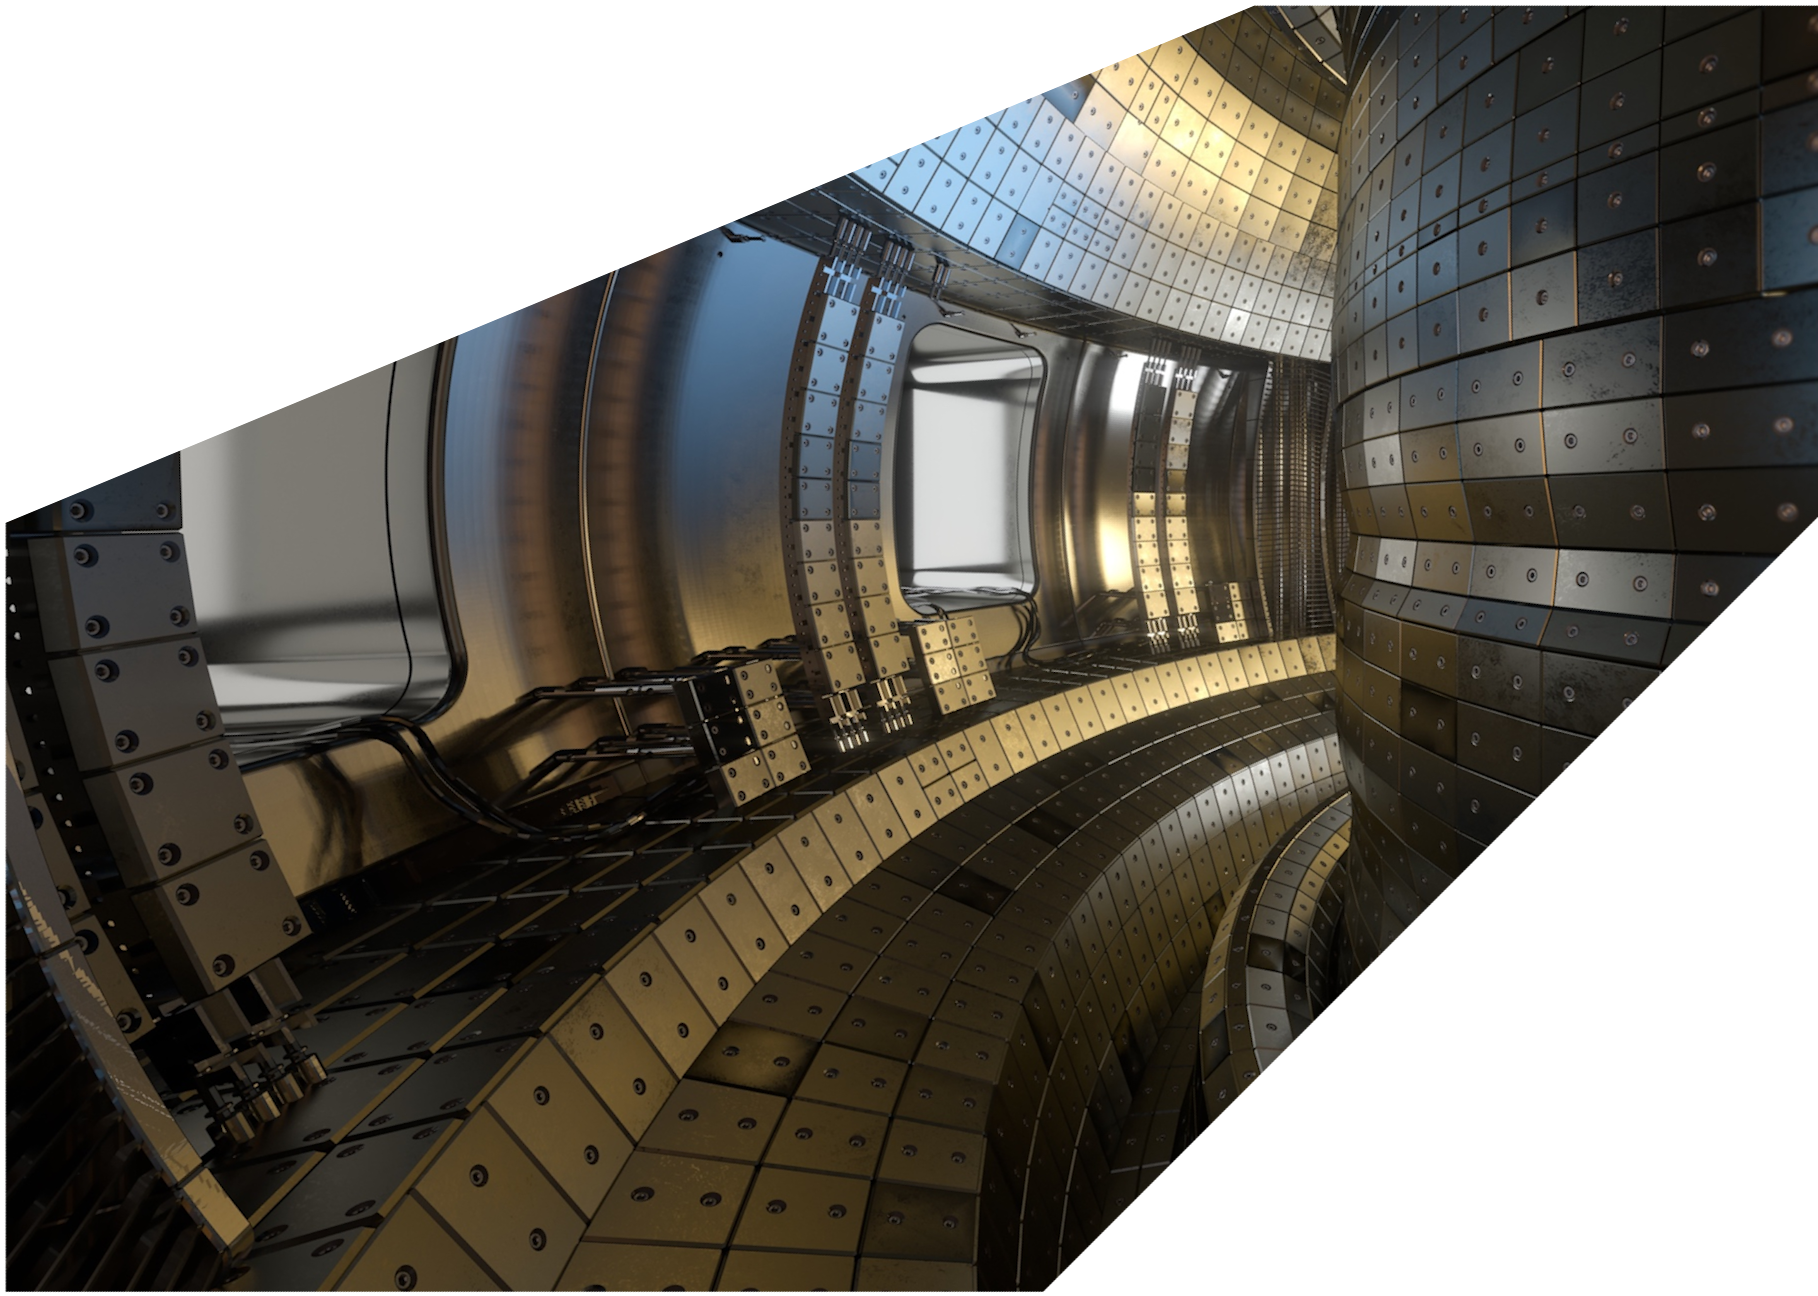
\includegraphics[width=0.9\textwidth]{../corpics/tokintcrop}}%<==omit
\end{titlepage}%<==omit

\hspace{-30mm}\begin{table}[h]
\sffamily
\begin{center}
\textbf{\textsf{UKAEA REFERENCE AND APPROVAL SHEET}}
\begin{tabular}{||p{5.7cm}|p{4.7cm}|p{5.0cm}||}
\hline
\hline
& Client Reference: &  \\
\hline
& UKAEA Reference: & \culhamshorttitle \\
& & \\
\hline
& Issue: & \culhamissueno \\
\hline
& Date: & \culhamdateb \\
\hline
\multicolumn{3}{||l||}{} \\
\multicolumn{3}{||l||}{Project Name: ExCALIBUR Fusion Modelling System} \\
\multicolumn{3}{||l||}{} \\
\hline
\end{tabular}
\begin{tabular}{||p{3.3cm}|p{4.6cm}|p{3.5cm}|p{3.6cm}||}
\hline
& Name and Department & Signature & Date \\
\hline
Prepared By: & \culhamauthora & N/A & \culhamdate \\
& \culhamauthor & N/A & \culhamdate \\
%& \culhamauthorb  & N/A & \culhamdate \\
%& \culhamauthorc  & N/A & \culhamdate \\
& & & \\
& BD & & \\
\hline
Reviewed By: & \culhamcontactname & 
\includegraphics[width=3.0cm]{../corpics/blanksign}& \culhamdatea \\
& & & \\
& Advanced Computing Dept. Manager & & \\
\hline
%Approved By: & \culhamboardname  & \includegraphics[width=3.0cm]{../corpics/mobsign} & \culhamdateb \\
%& & & \\
%& MSSC & &\\
%\hline
\hline
\end{tabular}
\end{center}
\end{table}


\clearpage
\section{Introduction}\label{sec:intro}
Rather than attempting to develop a fully 3-D Exascale targeted plasma edge (or 
boundary) code from day one, project \nep \   will first focus upon the 
development of ``\papp s"~\cite{proxies}, developed by partners across 
the project through a series of Grant calls. These must be designed and encoded 
to pave the way to the fully 3-D, actionable and performant \nep \   code (or 
codes) outlined in the Science Plan. As such, all \nep \   \papp s must 
capture the functionality and performance/scalability characteristics of the 
eventual infrastructure as much as possible. In addition, all of the solutions 
across the \nep \   programme must eventually be synergistic, leading to an  
integrated solution for the eventual code(s) -- this will require close 
cooperation through co-design across all partner organisations. The baseline 
\papp s for the initial years of the project are described briefly in the 
Science Plan~\cite{sciplan}, and expanded upon below to give the
``baseline plan" model equations, geometry and boundary conditions.
Note, the baseline plan does not preclude additional 
functionality that any bidder may deem useful (or even essential) to the 
project. Bidders are encouraged in their response to calls to be creative 
and ambitious and to describe their own ideas and plans for delivering above 
and beyond core scope,  provided the aim is 
to increase impact, quality, reduce risk and/or accelerate delivery (and that 
deliverables are fully aligned with the goals of the \nep \   Science Plan~\cite{sciplan}).

%For each \papp\ , bidders should describe their approach (including their 
%initial thoughts around provisional selection for algorithm and library 
%options), programming language preference etc. (which will be down selected in 
%negotiation with UKAEA) and should indicate how their solution will in the 
%eventual \nep \   code deliver:
%\begin{itemize}
%\end{itemize}
%\item[a)] Code sustainability.
%\item[b)] Easy to deploy, easy to use and easy to develop code.
%\item[c)] Performance (both strong and weak scaling).
%\item[d)] Performance portability (targeting multiple candidate Exascale 
%architectures).
%\item[e)] Actionable solutions (UQ).
%\item[f)] Quality, through rigorous Verification and Validation procedures.
%\item[g)] The ability to generate surrogate models derived from the code (eg.\ 
%through Model Order Reduction).

At baseline, \papp s target $x86$ (and ideally IBM POWER and ARM 
CPU) architectures (multi-core and multiple node) for scalability to first 
generation Exascale hardware. \Papp s might also target other 
Exascale candidate architectures (eg.\ GPGPU) and/or demonstrate a capability to 
explore the use of novel hardware as it becomes available to the \exc \   
project as part of the novel test-bed programme. In order to execute
efficiently on parallel architectures, \papp s are expected to examine
use of MPI, OpenMP or some other software technology
(ideally with a focus upon performance portability).

%If a bidder determines there 
%is insufficient resource to do so (or if they do not possess the relevant 
%skills), they should instead indicate that they are willing to work closely 
%with other \nep \   team members who have demonstrated skills in accelerator 
%exploitation.
%In order to target the chosen architecture(s), it will be necessary 
%indicate whether they intend to deploy MPI and OpenMP or some other 
%-- including a clear explanation as to why (and be prepared to negotiate with 
%UKAEA).

Supporting information regarding Braginskii's transport
coefficients for plasma in a strong magnetic field appears in \Sec{bragin}.
A description of sources of atomic and molecular radiation is given as an
annex in \Sec{atomic}.

\subsection{Overall Plan}\label{sec:plana}
In the Science Plan~\cite{sciplan} the description of work 
extending beyond Y3 (early 2022) is deliberately vague on the subject of ``gyrokinetics'', as no
widely accepted model for the tokamak edge appears to be available as of early~Y2,
and even should one appear, it might not be suitable for use in~Y3 in~\nep.

As listed, the \papp s correspond to Plan~A, which assumes that no suitable gyroaveraged
model will emerge in time, hence \emph{kinetic} implies Particle-in-Cell~(PIC).
PIC  approaches, where charge conservation
is vital to control errors, can anyway usefully be pursued
for modelling low collisionality plasma species, and should simplify nicely to 
treat neutral species with long mean-free-paths in tokamak edge problems
where mass conservation has been discovered to be
critical. Moreover in the context of classical fluid dynamics, 
the transition from fluid to particles, or short to long mean-free-path,
has been well-studied because of the
application to the space vehicle re-entry problem and related hypersonic situations.
Thus the hybrid fluid/PIC approach
might be regarded as a relatively low-risk route to achieving a robust
numerical algorithm.

Evidently full-orbit PIC has the potential to be extremely inefficient relative to 
gyroaveraged kinetic theory because of the need to follow gyro-orbits in detail. Hence
if this can be avoided, either through gyroaveraging or clever numerics or indeed
a combination of both,
then Plan~B will see \emph{kinetic} imply gyroaveraged kinetic theory for modelling plasma species
in the \papp s.

Regarding implementation at the Exascale there is also a
conservative Plan~A approach which sees the
use of relatively simple data structures such as scalar and vector arrays to transfer
data, and consequent use of existing code-coupling technologies.
Plan~B is an aggressive approach to implementation which sees
custom data structures allowing for all physical data (particle arrays
and fluid field vectors) colocated near a point to be
held close in memory, permitting very tight custom code-coupling. As with the
\emph{kinetic} options, this Plan~B promises significantly faster solutions than
the corresponding Plan~A, but its adoption depends on the outcome of research work
to de-risk.


\subsection{\Papp s Summary}\label{sec:papp}
%The description of the \papp s in the Science Plan is inevitably
%terse and that in the document ``Equations for \exc/\nep \ \papp s"~\cite{pappeqs}
%is inevitably focussed on the mathematics.
%This appendix elucidates
%thinking behind their choice and the priorities for their implementation.

The overall thinking behind the \papp s is to explore potential `roadblocks' to the Exascale as
early and in as simple a context as is possible, beginning with algorithmic
roadblocks. \nep \ is directed towards producing `actionable' code as the basis
for large procurements, whereas
more physics-focussed software projects conducted by the
worldwide nuclear fusion have already advanced to greater complexity,
minimising the risk that unexpected problems will appear in the full model.
%is minimised by competing fusion software projects that will have `rushed in'
%to greater complexity, cf.\ the business adage that ``it is better to be second first".)

The numbering of \papp s below corresponds to the Science Plan.
\begin{itemize}
\item[2-1] 2-D model of anisotropic heat transport. It is important to determine early the
degree of anisotropy that high-order elements can treat without special coding. If this 
is unsatisfactorily small, then there are implications for geometry input as well as
algorithmic developments that are best addressed as early as possible.
\item[2-2] 2-D elliptic solver in complex geometry. One of the indicated elliptic solvers is
Grad-Shafranov to produce high order (`spectrally') accurate magnetic fields for
use in many other \papp s. Since Sovinec~\cite{Ho14Solv} has already produced a spectral element
Grad-Shafranov code, the corresponding \nep\ development should mainly serve to
identify practical issues concerning implementing high order fe models. The second
solver additionally presents a chance to explore comparatively novel meshing techniques developed under
Activity~A2.1, and later the preconditioning techniques of A2.7.
\item[2-3] 1-D fluid solver with simplified physics but with UQ and realistic boundary conditions.
This will determine the capability of spectral/hp element to handle sonic outflow
boundary conditions needed to represent sheaths, together with large source terms, as well
as identifying practical issues concerning intrusive UQ. This software is already
potentially useful in its own right for example in modelling MAST-U divertor,
and other workers might be drawn in to add additional physical effects to this end.
\item[2-4] Spatially 1-D plasma model incorporating velocity space effects. From the
numerical analytic point-of-view, this is a key demonstration of spectral/hp element capability to
handle particle interactions. % within the \emph{volume}.
However, again this could be a basis for divertor modelling,
to explore sheath effects depending on fieldline incidence on surface, and with minor
modification the spread of particle energy around tile edges and corners as performed
by Gunn~et~al~\cite{Gu19Stud,De19Phys} for ITER application.
\item[2-5] Spatially 1-D multispecies plasma model. Multispecies
throws up a surprising
number of issues concerning data definitions (eg.\ changes to the Coulomb
logarithm), structures to deal with different number of species, and perhaps most
significantly, complicated inter-species interaction terms both within
and at the domain boundaries. This is also an opportunity to mix fluid and
\emph{kinetic} representations of \emph{different} species  within the \emph{volume}.
\item[2-6] Spatially 2-D plasma model incorporating velocity space effects. 
With the 1-D multispecies fluid work's having made the generalisation to 2-D
straightforward, the challenge here is to start writing a complex \papp \
in production mode, incorporating the research put into design, documentation,
code generation and benchmarking. There is an opportunity to study species
with both fluid and \emph{kinetic} representations depending on location relative
to the wall. Again this is potentially a useful tool in its
own right, capable of revealing deficiencies in previous 2-D modelling work.
\item[2-7] Interaction between models of different dimensionality.
This should verify that the design has the right data structures to handle additional further
complexity beyond intrusive and ensemble-based UQ and model order reduction. The hopefully 
burgeoning \nep \ community
could develop this into a design tool with a capability both to explore a large
area of tokamak edge parameter space quickly in 0-D or 1-D and also to focus on
relatively small but critical 2-D features, such as tile edges.
\item[2-8] Spatially 3-D plasma \emph{kinetic} models.
These will represent the full fluid model
produced by the 5-year \nep \ project, incorporating features of 2-D fluid and
\emph{kinetic} work in a 3-D code.
\end{itemize}
\begin{itemize}
\item[3-1] 2-D particle-based model of neutral gas \& impurities with critical physics.
This will be a $2d3v$~code (ie.\ spatially 2-D distribution of particles
with $3$~velocity components)
designed from the outset to interact with a high-order finite-element fluid model of plasma.
It gives an opportunity to check out ideas on optimal usage of particles.
\item[3-2] 2-D moment-based model of neutral gas \& impurities.
Constructing a 2-D fluid code of neutral gas from the Nektar++ software should be
a valuable educational exercise, whilst providing scope for cross-validating the 2-D particle model.
\item[3-3] Interaction with 2-D plasma model when available.
Building on the 1-D multispecies fluid work, the challenge here is to incorporate
in the fluid code of \Papp \ PA2-6, particle effects from PA3-1, which will in
the higher dimensional space be more subject to lack of numerical
resolution or `noise'. Should PA3-3 be accelerated, it could usefully 
treat both plasma and neutrals via particle models.
\item[3-4] 3-D model of neutral gas \& impurities.
This is now at full dimensional complexity, incorporating selected ideas 
on optimal usage of particles.
\item[3-5] Interaction with 3-D plasma model.
This will represent the full model produced by the 5-year \nep \ project,
a coupling of fluid and \emph{kinetic} software developed under the FM-WP2 work-package as PA2-8,
incorporating features of \Papp s 3-1 to 3-4, and allowing for additional input from PA3-6.
\item[3-6] Staged introduction of additional neutral gas/impurity physics.
It is expected that the \nep \ community will join in to supplement
the software with a wide-ranging capability to treat a wide range of additional 
nuclear, atomic and molecular effects.
\end{itemize}


%Note: Work extending beyond Y3 is deliberately vague on the subject of gyrokinetics, as no
%widely accepted model for the tokamak edge appears to be available as of early~Y2,
%and even should one appear, it might not be suitable for use in~Y3 in~\nep.


\section{Braginskii coefficients}\label{sec:bragin}
Braginskii's transport coefficients are widely used in tokamak edge modelling.
Object-oriented Fortran code to compute the Braginskii coefficients is available
at \\
{\tt https://github.com/wayne-arter/smardda-misc.git}.

\subsection{General}\label{sec:general}
Note that $k_B T(\mbox{units of }K) = |e| T(\mbox{units of }eV)$ where $k_B$ is Boltzmann's constant and $|e|$ is the
absolute value of the charge on the electron. Otherwise suffix~$B$ denotes a quantity
from the Plasma Formulary~\cite{NRLpf07}. See also Braginskii's paper~\cite{Br65Tranwarv}.
The subsequent corrections by Epperlein and Haines, and by Mikhailovski and Tsypin are not relevant to this work.

In a magnetic field, the direction of which is given by unit vector~${\bf b}$,
Goedbloed and Poedts~\cite{goedbloedpoedts} define three auxilliary vectors for
a vector~${\bf v}$, viz.
\begin{equation}\label{eq:vaux}
{\bf v}_{\parallel}= {\bf b} ({\bf b} \cdot {\bf v}), \;\; {\bf v}_\wedge= {\bf b} \times {\bf v}
\;\;\mbox{and}\;\; {\bf v}_\perp=({\bf b} \times {\bf v} ) \times {\bf b}
\end{equation}
If ${\bf v} = (v_1, v_2, v_\parallel)$ and ${\bf b}$ is aligned with the 3-axis
in a Cartesian coordinate system, then
\begin{equation}\label{eq:vpt}
{\bf v}_{\parallel}= (0,0,v_\parallel), \;\; {\bf v}_\wedge= (-v_2,v_1,0)
\;\;\mbox{and}\;\; {\bf v}_\perp=(v_1,v_2,0)
\end{equation}
It may be shown that a tensor~$\mathcal{T}$ which is symmetric under rotation
about~${\bf b}$ has the form (in Cartesians) 
\begin{equation}\label{eq:tensor}
\mathcal{T}=
\begin{pmatrix} \mathcal{T}_\perp & - \mathcal{T}_\wedge & 0 \\
 \mathcal{T}_\wedge &  \mathcal{T}_\perp & 0 \\
 0 & 0 & \mathcal{T}_\parallel \\
\end{pmatrix}
\end{equation}
so that
\begin{equation}\label{eq:TV}
\mathcal{T} \cdot {\bf v} = \mathcal{T}_\parallel {\bf v}_\parallel + \mathcal{T}_\wedge {\bf v}_\wedge + \mathcal{T}_\perp {\bf v}_\perp
\end{equation}

\subsection{Conduction, Viscous and Resistive Coefficients}\label{sec:coefficient}
The electron parallel thermal conductivity in the Braginskii theory is given as~\cite{NRLpf07}
\begin{equation}\label{eq:kapbae}
\kappa^e_{B\|}= 3.2 \frac{Nk_BT_e}{m_e} \tau_e
\end{equation}
a formula valid in either cgs or SI units, where $\tau_e$ is 
the electron relaxation time (measured in seconds), defined below.
The notation is standard, with $N$ the number density of electrons, approximately 
the same as the number density of ions, $m_e$ the electron mass, and $T_\alpha,\;\;s=i,e$
the temperature of species~$\alpha$.
The perpendicular electron thermal conductivity satisfies
similarly
\begin{equation}\label{eq:kapberpe}
\kappa^e_{B\perp}= 4.7 \frac{Nk_BT_e}{m_e} \tau_e \cdot \frac{1}{(\omega_{ce}\tau_e)^2}
\end{equation}
where the electron cyclotron frequency
\begin{equation}\label{eq:cyce}
\omega_{ce}= \frac{e}{m_e}\cdot B
\end{equation}
Equivalent expressions for ions are
\begin{equation}\label{eq:kapbai}
\kappa^i_{B\|}= 3.9 \frac{Nk_BT_i}{m_i} \tau_i
\end{equation}
\begin{equation}\label{eq:kapberpi}
\kappa^i_{B\perp}= 2 \frac{Nk_BT_i}{m_i} \tau_i \cdot \frac{1}{(\omega_{ci}\tau_i)^2}
\end{equation}
where the ion cyclotron frequency
\begin{equation}\label{eq:cyci}
\omega_{ci}= \frac{ZeB}{m_i}= \frac{e}{m_p} \cdot \frac{ZB}{A}
\end{equation}
where $Z$ is the charge state of the ion and $A$ its atomic mass.
The definitions above have to be interpreted in the context of the
equations given in~\cite{NRLpf07}, so that thermal diffusivities are
obtained by dividing by~$3n_\alpha/2$ where $\alpha=i,e$ is the species index.
It is also convenient to introduce the dimensionless factors
\begin{equation}\label{eq:xe}
x_e= \omega_{ce}\tau_e
\end{equation}
\begin{equation}\label{eq:xi}
x_i= \omega_{ci}\tau_i
\end{equation}

Kinematic viscosities in the Braginskii theory may be taken as
\begin{equation}\label{eq:nuparae}
\nu^e_{\|}= 0.73 Nk_BT_e \tau_e /(N m_e) = 0.73 \frac{k_BT_e}{m_e} \tau_e
\end{equation}
\begin{equation}\label{eq:nuperpe}
\nu^e_{\perp}= 0.51 Nk_BT_e \tau_e /(N m_e) \frac{1}{x_e^2}= 0.51 \frac{k_BT_e}{m_e} \tau_e\frac{1}{x_e^2}
\end{equation}
\begin{equation}\label{eq:nuparai}
\nu^i_{\|}= 0.96 Nk_BT_i \tau_i /(N m_i) = 0.96 \frac{k_BT_i}{m_i} \tau_i
\end{equation}
\begin{equation}\label{eq:nuperpi}
\nu^i_{\perp}= 0.3 Nk_BT_i \tau_i  /(N m_i)\frac{1}{x_i^2} = 0.3 \frac{k_BT_i}{m_i} \tau_i\frac{1}{x_i^2}
\end{equation}


Key quantities in the calculation of all these terms are $\tau_\alpha$, $\alpha=i,e$.
The first step in their calculation is to convert their formulas,
usually given in cgs, to SI units, giving
\begin{equation}\label{eq:tauesi}
\tau_e=6 \sqrt{2\pi^3} \frac{\epsilon_0^2\sqrt{m_e}}{e^4} \frac{(k_BT_e)^{3/2}}{Z^2 N \Lambda}
=3.44 \times 10^{-7} \frac{(T_e)^{3/2}}{Z^2 (N/10^{18}) \Lambda}
\end{equation}
\begin{equation}\label{eq:tauisi}
\tau_i=12 \sqrt{\pi^3} \frac{\epsilon_0^2\sqrt{m_p}}{e^4} \frac{(k_BT_i)^{3/2} \sqrt{A}}{Z^4 N \Lambda}
=2.09 \times 10^{-5} \frac{(T_i)^{3/2} \sqrt{A}}{Z^4 (N/10^{18}) \Lambda}
\end{equation}
where the notation is standard, except possibly the use of $\Lambda$ for
the Coulomb logarithm. The above check with expressions in Wesson~\cite[\S\,14]{wesson}.
Note that $Z^2 \tau_i$ differs from~$\tau_e$ in being larger by  a factor of $\sqrt{2m_i/m_e}\approx 60 \sqrt{A}$
(also substituting $T_i$ for~$T_e$ is necessary). The factors in~$Z$ are taken from the
original Braginskii paper~\cite{Br65Tranwarv}.

It follows that the $x_\alpha$ factors may be conveniently written
\begin{equation}\label{eq:xen}
x_e =6.05 \times 10^{4} \frac{(T_e)^{3/2} B}{Z^2 (N/10^{18}) \Lambda}
\end{equation}
\begin{equation}\label{eq:xin}
x_i =1997 \frac{(T_i)^{3/2} B}{Z^3 (N/10^{18}) \sqrt{A} \Lambda}
\end{equation}
The large coefficients in \Eqs{xen}{xin} explain why classical transport is
so anisotropic.

Substituting the explicit expression for $\tau_e$ in \Eqs{kapbae}{kapbai} gives
respectively, the thermal parallel diffusivities are
\begin{equation}\label{eq:kappae}
\kappa_{e\|}= 13 \sqrt{2\pi^3} \frac{1}{\sqrt{m_e}}\frac{\epsilon_0^2}{e^4} \cdot
\frac{(k_BT_e)^{5/2}}{Z^2 N\Lambda}
\end{equation}
\begin{equation}\label{eq:kappai}
\kappa_{i\|}= 16 \sqrt{\pi^3} \frac{1}{\sqrt{m_p}}\frac{\epsilon_0^2}{e^4} \cdot
\frac{(k_BT_i)^{5/2}}{Z^4 N\Lambda \sqrt{A}}
\end{equation}
and the ratios are
\begin{equation}\label{eq:xee}
x_e=\frac {6 \sqrt{2\pi^3}\epsilon_0^2} {\sqrt{m_e}e^3} \cdot
\frac {(k_BT_e)^{3/2}B} {Z^2 N\Lambda}
\end{equation}
\begin{equation}\label{eq:xie}
x_i=\frac {12 \sqrt{\pi^3}\epsilon_0^2} {\sqrt{m_p}e^3} \cdot
\frac{(k_BT_i)^{3/2}B} {Z^3 N\Lambda \sqrt{A}}
\end{equation}
An expression for the perpendicular ion conductivity, maintaining
the fixed physical factors is of interest
\begin{equation}\label{eq:kperpie}
\kappa_{i\perp}=\frac{e^2\sqrt{m_p}}{9 \sqrt{\pi^3}\epsilon_0^2} \cdot
\frac{Z^2 N\Lambda \sqrt{A}}{(k_BT_i)^{1/2}B^2}
\end{equation}
Assuming $T_i$ is measured in~$eV$, and $N$ in units of $10^{18}$\,m$^{-3}$, then
\begin{equation}\label{eq:kperpin}
\kappa_{i\perp}=6.67 \times 10^{-4} \cdot
\frac{Z^2 (N/10^{18}) \Lambda \sqrt{A}}{(T_i)^{1/2}B^2}\;\;m^2 s^{-1}
\end{equation}
and
\begin{equation}\label{eq:kperpen}
\kappa_{e\perp}=5.26 \times 10^{-5} \cdot
\frac{Z^2 (N/10^{18}) \Lambda}{(T_e)^{1/2}B^2}\;\;m^2 s^{-1}
\end{equation}

The plasma resistivity is taken as
\begin{equation}\label{eq:resis}
\eta=\eta_B/\mu_0 =\frac{0.51\sqrt{m_e}e^2}{6 \sqrt{2\pi^3}\mu_0\epsilon_0^2} \cdot
\frac{Z \Lambda}{(k_BT_e)^{3/2}}
\end{equation}
Assuming $T_e$ is measured in~$eV$, then
\begin{equation}\label{eq:resisn}
\eta=\eta_B/\mu_0 =41.9\cdot\frac{Z \Lambda}{(T_e)^{3/2}}\;\;m^2 s^{-1}
\end{equation}


\subsection{Prandtl Numbers}\label{sec:prandtl}
The above expressions (except for the resistivity) apply strictly only when there
are separate equations for ion and electron transport, 
so decisions have to be taken about how to combine the transport coefficients
to treat the plasma as a single fluid. For the thermal transport, since 
pressures $p_e\approx p_i$, it is sufficient to add the $\kappa_\alpha$. However, the values for ions and electrons
are so disparate because $m_p\gg m_e$ that one or other might be neglected, 
assuming~$B$ is of order unity (in Tesla) and $T_e\approx T_i$, 
thus $\kappa_{e\|} \gg \kappa_{i\|}$ and hence 
$\kappa_{\|}\approx \kappa_{e\|}$, since 
\begin{equation}\label{eq:rbrat}
\left(\frac{x_i}{x_e}\right)^2 = \frac{2m_e}{Z^2 A m_p} \left(\frac{T_i}{T_e}\right)^3
\end{equation}
It also follows that
\begin{equation}\label{eq:krat}
\frac{\kappa_{e\perp}}{\kappa_{i\perp}} = 0.078 \left(\frac{T_i}{T_e}\right)^{1/2}
\frac{1}{\sqrt{A}}
\end{equation}
thus $\kappa_{\perp}\approx \kappa_{i\perp}$.
There is the caveat that if $T_i$ is approximately spatially constant radially,
then $\kappa_{e\perp}$ might become relevant.

As for viscosity, since the ion momentum is so much greater than the electron momentum, then $\nu\approx\nu^i$.

For interchange motions where flows are perpendicular to the field, take 
$\kappa=\kappa_{i\perp}$, then on the \emph{Cambridge} definition, the magnetic Prandtl number is
\begin{equation}\label{eq:zeta}
\zeta=\frac{\eta}{\kappa_{i\perp}}=\frac{0.765}{\sqrt{2}}\frac{1}{\mu_0}\sqrt{\frac{m_e}{m_p}} \cdot
\frac{B^2}{Z N\sqrt{A}} \frac{(k_BT_i)^{1/2}}{(k_BT_e)^{3/2}}
\end{equation}
which evaluates as ($T_\alpha$ in~$eV$, $N$ in units of $10^{18}$\,m$^{-3}$)
\begin{equation}\label{eq:zetan}
\zeta=\frac{\eta}{\kappa_{i\perp}}=62\,700 \cdot \frac{B^2}{Z (N/10^{18})\sqrt{A}} \frac{(T_i)^{1/2}}{(T_e)^{3/2}}
\end{equation}
It may be argued that it is more appropriate to use the `anomalous'  value of $1\,m^2 s^{-1}$,
in which case \Eq{resisn} without units gives the `Cambridge'  magnetic Prandtl number.

The usual Prandtl number is
\begin{equation}\label{eq:sigma}
\sigma=\frac{\nu_{i\perp}}{\kappa_{i\perp}}=0.23
\end{equation}
Note that P.H.Roberts~\cite{roberts} defines the magnetic Prandtl number
as $\nu/\eta=\sigma/\zeta$, and his definition is more widely used.


\clearpage
\section{System 2-1: 2-D model of anisotropic heat transport} \label{sec:sys2-1}
The model for time evolution of the temperature field~$T$ is thermal diffusion,
which in a plasma gives
\begin{equation}\label{eq:plas2diff}
\frac{3}{2} N \frac{\partial T}{\partial t}=\nabla \cdot \mathcal{K}  \nabla T
\end{equation}
where the thermal conductivity tensor is $\mathcal{K}$.
(Compare the model for a solid
\begin{equation}\label{eq:solidiff}
\rho_m c_p \frac{\partial T}{\partial t}=\nabla \cdot k_c \nabla T
\end{equation}
where the thermal conductivity tensor is $k_c$, $\rho_m$ is the mass density of the medium 
and $c_p$ is its specific heat at constant pressure, implying
that the thermal diffusivity tensor is $\kappa=k_c/\rho_m c_p$.)
Introducing vector components as  in \Sec{intro},
thermal diffusion in a plasma after Braginskii is thus
\begin{equation}\label{eq:plas2brag}
\frac{3}{2} N \frac{\partial T}{\partial t}=
\nabla \cdot \left(
\mathcal{K}_{\|} {\bf b} [{\bf b}.\nabla T] +
\mathcal{K}_{\perp} (\nabla T - {\bf b} [{\bf b}.\nabla T])+
\mathcal{K}_{\wedge} {\bf b} \times \nabla T
\right) 
\end{equation}

Henceforth, the `wedge' transport ie. in due to the term in $\mathcal{K}_{\wedge}$
is neglected for the reason that it may be rearranged to give
a convection-like term, via the identity 
\begin{equation}\label{eq:crossxp}
\nabla \cdot \mathcal{K}_\wedge {\bf b} \times \nabla T = \nabla \cdot ({\bf u}_\wedge  T)
\end{equation}
where
\begin{equation}\label{eq:uxp}
{\bf u}_\wedge = \nabla \times (\mathcal{K}_\wedge {\bf b})
\end{equation}
(In any event, if $\mathcal{K}_\wedge$ is a function purely of~$T$, and
$\nabla \cdot {\bf b}=\bf{0}$, then the terms in \Eq{crossxp} vanish.)

Expressions for the thermal diffusivities $\kappa_{\perp}$ and~$\kappa_{\|}$ for
the different species
are given in \Sec{coefficient}, where they incorporate  the factor $\frac{3}{2} N$,
ie.\ $\kappa_{(\perp , \|) e,i}=\mathcal{K}_{(\perp, \|)}/(\frac{3}{2} N)$.

\subsection{Test Cases}\label{sec:tests}
The aim of the work is to calculate in a series of calculations that increasingly
approach the realistic model, the magnitude of the spurious numerical diffusion
perpendicular to the magnetic field direction~${\bf b}$. The main interest concerns
how much diffuses in the plasma, not the solid surface, even though the deposition
of power is on the surface, reason: all sorts of complicated extra physics come
into play in the plasma especially near surfaces.
\subsubsection{Starting Case}\label{sec:start}
For the 2-D test case illustrated in \Fig{aniso}, it is suggested that $\kappa_{\perp}=0$
so that any perpendicular diffusion is numerical in origin. Given this,
the problem can be analysed using any spatial scale and any convenient~$\kappa_{\|}$.
However an order of magnitude estimate for tile dimensions is one metre,
discharge timescale is one second upwards. For plasma properties
assume $N=10^{18}$\,m$^{-3}$, $T_i=T_e=10$\,eV, $Z=A=1$, $B=3$\,T and solid temperatures say $500^o$\,C.

In \Fig{aniso}, $T=T_0>0$ over the interval on the left hand boundary that is connected by field
in direction~${\bf b}$ with the thick red line,
elsewhere on the blue fieldlines, $T=0$. The red region lies on a black line
which denotes the boundary between anisotropic conductor and  perfect insulator. 
The exact steady-state solution has $T=constant$ along fieldlines, but numerical
diffusion will result in non-zero~$T$ in the region of blue fieldlines.
The relative size of this numerical diffusion must be estimated as a function
of incidence angle~$\theta$, where interest attaches to small $\theta\leq2^o$.
\begin{figure}
\centerline{
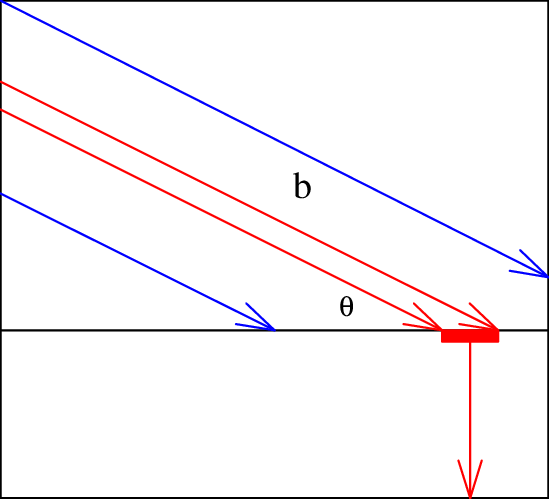
\includegraphics[width=8.0cm]{../png/aniso.png}
}
\caption{Sketch of the test configuration, showing fieldlines in direction~${\bf b}$
and the boundary between anisotropic conductor and perfect insulator.
\label{fig:aniso}}
\end{figure}

\subsubsection{Intermediate Case}\label{sec:intermediate}
To test curvature effects the whole 2-D domain of \Fig{aniso} could be distorted by conformal mapping
(which preserves angles).

\subsubsection{Realistic Case}\label{sec:realistic}
This needs to be 3-D and involve JET divertor tile descriptions derived from
the output of the CAD design tool, together with information
describing the magnetic field as a function of position, which will be supplied.
The magnetic equilibrium may be supplied analytically after Solovev, but the
usual input is as an .eqdsk file.
The EQDSK~G format is a ``non-standard" standard for
solutions $\psi(R,Z), p(\psi), I(\psi)$ of the Grad-Shafranov equation, where
$\psi$ is the magnetic flux and $(R,Z)$ are cylindrical coordinates
in planes normal to the toroidal direction. The functions~$p$ and~$I$ give the
variation of the pressure and toroidal field respectively.
The basic standard for EQDSK~G may be found at:
\url{https://fusion.gat.com/theory/Efitgeqdsk} (which may be password-protected)
or else at ~\url{https://w3.pppl.gov/ntcc/TORAY/G_EQDSK.pdf}
The flux~$\psi(R,Z)$ is sampled at uniformly spaced points on a direct product grid,
for which the .eqdsk header defines the mesh-size, as well as other useful
information, such as the flux on axis and at boundary.
Unfortunately the strict EQDSK~G standard uses a Fortran format that does
not require spaces between samples, hence there are many variants for
languages that cannot handle this situation, that have introduced other
features such as mistakes in field helicity, factors of $2\pi$ in the flux, etc.
Routines that calculate magnetic field~${\bf B}$ using cubic spline interpolation
could be made available. It would be desirable for the output of System 2-2
to be used.


\subsubsection{Extended Case}\label{sec:extended}
An extended test would allow for heat transfer in the solid surface sketched 
at bottom of \Fig{aniso}, taking say thermal diffusivity for Tungsten
$\kappa \approx 3 \times 10^{-5}$\,m$^2$ s$^{-1}$. 
%\begin{figure}
%\centerline{
%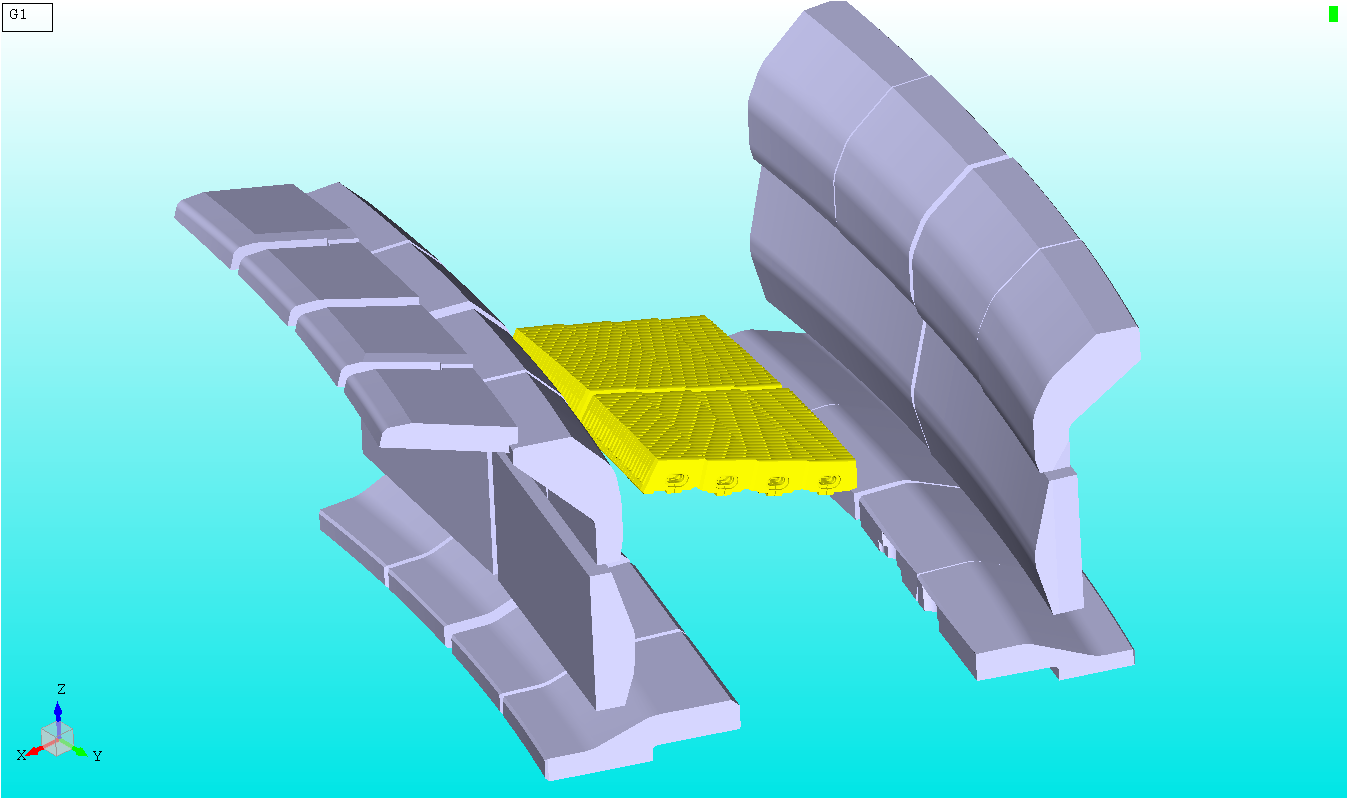
\includegraphics[width=8.0cm]{../png/pretty}
%}
%\caption{CAD for JET divertor after simplification. A $15^o$ sector in toroidal angle is shown,
%except for the T5~armour, where only $7.5^o$ are drawn. The magnetic field (not shown)
%is predominantly directed in the toroidal direction to achieve near grazing incidence.
%\label{fig:pretty}}
%\end{figure}

\clearpage
\section{System 2-2: 2-D elliptic solver in complex geometry} \label{sec:sys2-2}
The geometry will be representative of a tokamak cross-section, possibly
omitting
the region containing the central hot plasma, so that topologically it
will be at most as complex as an annulus (one-hole). \Fig{xsect}
provides an example. 
The Last Closed Flux Surface~(LCFS) may be parameterised by arc-length
in the cross-sectional plane of projection.

\begin{figure}
\centerline{
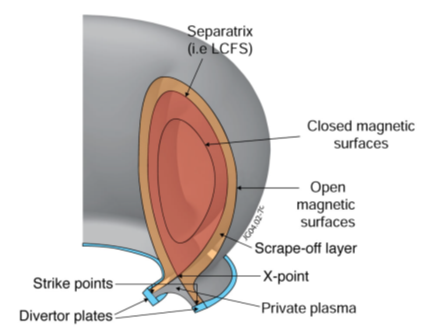
\includegraphics[width=8.0cm]{../png/xsect}
}
\caption{Sketch of the test configuration, showing tokamak cross-section
and the boundary of the Last Closed Flux Surface (LCFS).
\label{fig:xsect}}
\end{figure}

The elliptic equations to be considered now follow.

\subsection{Simplified Grad-Shafranov equation} \label{sec:GSimp}
This elliptic equation is a simplified version
of the Grad-Shafranov equation, see \cite{Ap18Equi}
\begin{equation}\label{eq:gs}
R^2 \nabla \cdot \frac{1}{R^2} \nabla \psi = -2 \mu_0 R J_{\phi}
\end{equation}
where $\psi$ is the poloidal magnetic flux and $(R,Z)$ are cylindrical coordinates
in planes normal to the toroidal direction~$\phi$, with the toroidal current
\begin{equation}\label{eq:jphi}
J_\phi= R \frac{dp(\psi)}{d\psi}+ \frac{I}{\mu_0 R} \frac{dI(\psi)}{d\psi} + J_{ext}(R,Z)
\end{equation}
The functions~$p$ and~$I$ give the variation as functions of~$\psi$
of the pressure and toroidal field respectively, and $J_{ext}(R,Z)$
may be produced in several ways, of which the commonest is by
poloidal field circuits, ie.\ localised current sources in cross-section.
Note that the operator in \Eq{gs} simplifies to
\begin{equation}\label{eq:gsimp}
\frac{\partial^2}{\partial R^2} - \frac{1}{R}  \frac{\partial}{\partial R} + \frac{\partial^2}{\partial Z^2}
\end{equation}
which implies that mathematically, $\psi$ satisfies a steady-state 2-D advection-diffusion
equation corresponding to unit diffusivity in the flow $u_R=1/R$.

To provide the simple test case, take $J_\phi=J_{ext}$ only with localised current sources.
The boundary conditions are $\psi=0$ on the LCFS
and $\psi \propto 1/\sqrt(R^2+Z^2)$ as $R,\;Z \rightarrow \infty$.

Note that the Grad-Shafranov equation has been solved using spectral elements by
others, eg.\ Sovinec~\cite{Ho14Solv}.
%so that $\psi$ decreases outwards from the LCFS

\subsection{Simplified non-Boussinesq vorticity equation} \label{sec:boussimp}
A simplified version of the non-Boussinesq vorticity equation to be solved for
the scalar field $\Phi(R,Z)$ in cylindrical polar coordinates~$(R,Z)$ is
\begin{equation}\label{eq:ellsimp}
\nabla_\perp \cdot \left( \frac{1}{B^2}  \nabla_\perp \Phi \right) = n
\end{equation}
where $B=|{\bf B}|$ is the amplitude of the imposed magnetic field,
density~$n$ acts as a source term, and the elliptic is to be solved
for~$\Phi$, subject to boundary conditions $\Phi=0$. The operator $\nabla_\perp$,
ignoring the components of magnetic field directed within the $(R,Z)$~plane,
reduces to the usual gradient~$\nabla$ in cylindrical polars of axisymmetric
fields, hence mathematically \Eq{ellsimp}
is equivalent to~\Eq{gs}.

$n$ will be set so that $n=n_0(s_i)$ on the boundaries,
where arc-length~$s_i$
parameterises the inner boundary if $i=1$ and the outer if $i=2$.
$n$ and $|B|$ will be specified functions of $(R,Z)$ that capture features
of the number density~$n$ distribution and magnetic field intensity distribution
expected in a tokamak,
Ideally $|B|$ would represent a solution of the Grad-Shafranov equation from \Sec{GSimp}.

\clearpage
\section{System 2-3: 1-D fluid solver with simplified physics but with UQ and realistic boundary conditions} \label{sec:sys2-3}
\subsection{Plasma Equations}\label{sec:sys23plas}
It is assumed that the single spatial dimension of the problem
corresponds to the arc length distance along a fieldline.
Starting from the two-fluid model of Braginskii~~\cite{Br65Tranwarv},
a set of equations resembling those of classical (compressible) hydrodynamics
may be derived by summing Braginskii's equations for number density,
momentum and energy.
Using the notation of ref~\cite{Ha13Benc}, introducing $T_d=T_i+T_e$,
neglecting the stress tensor terms (implicitly setting $\delta p_i=0$),
and assuming $B$ is independent of time, the resulting system is
\begin{eqnarray}\label{eq:sysn1}
U_d \frac{\partial}{\partial t} (N/B)+ 
\frac{\partial}{\partial s} (N U/B)&=&\frac{L_s S^n}{B} \\
U_d \frac{\partial}{\partial t} (N U/B)+ 
\frac{\partial}{\partial s} (N U^2/B)&=&
-\frac{1}{m_i B}\frac{\partial}{\partial s} (P_i + P_e) +\frac{L_s S^u}{m_i B} \label{eq:sysu1}\\
U_d \frac{\partial}{\partial t}\left( \frac{3}{2}(N kT_d/B)+
\frac{1}{2} (N U^2/B) \right) &+&\\
\frac{\partial}{\partial s} \left( \frac{5}{2}(N U kT_d/B) +
\frac{1}{2} (N U^3/B) \right) &=&
-\frac{1}{m_i B}\frac{\partial}{\partial s} (q_i + q_e) +
\frac{L_s (S_i^E+S_e^E)}{m_i B} \label{eq:syst1}
\end{eqnarray}
where 
\begin{equation}\label{eq:hs}
L_s= \frac{\partial s_{\parallel}}{\partial s}
\end{equation}
$U_d =L_s/t_0$ is a speed measuring the importance of the transient term, $s$ parameterises
distance along the fieldline,
%temporarily the conduction term in $(q_i + q_e)$ has been retained,
and some variables from~\cite{Ha13Benc} have been promoted to capitals to 
indicate that they retain their physical dimensions.
For the case of a fieldline connecting two walls at $s=\pm L$, 
\begin{equation}\label{eq:spar}
s_{\parallel}=L(2s-1)
\end{equation}
and so $L_s=2L$.
The constant $k$ is such that
\begin{equation}
k= \frac{k_B}{m_i}\;\;\mbox{or}\;\;k=\frac{|e|}{m_i}
\end{equation}
where $k_B$ is Boltzmann's constant and $|e|$ is the unit of charge, depending whether T is measured in Kelvin or~$eV$. 
Note that in adding Eqs.(3) and~(4) of~\cite{Ha13Benc}, equipartition and collision terms cancel 
to give \Eq{syst1}. The perfect gas equation of state will be assumed, so that
\begin{equation}\label{eq:sysp}
\frac{p_i+p_e}{m_i}=N k T
\end{equation}


The boundary conditions are that $|U|=|M_s| C_S$ at $s=0,1$ where the sound speed
\begin{equation}
C_S= \sqrt{kT_d}
\end{equation}
and $|M_s|$ is the Mach number, since $M_s$ will be allowed to take either sign. Normally $|M_s|=1$
so that $M_0=-1$ and $M_1$=1 where the subscript corresponds to value of~$s$.
The combined energy flux at each boundary has
\begin{equation}
|Q_{\parallel}|=m_i C_S N (\delta_e kT_e + \delta_i kT_i) \approx
m_i C_S N \delta kT_d
\end{equation}
if $\delta \approx \delta_e \approx \delta_i$. For definiteness, $\delta=\frac{1}{2}(\delta_e+\delta_i)$
will be assumed.

\subsection{Fluid Equations with Sources}\label{sec:sys23fluid}
It is convenient to replace the source terms in \Eqr{sysn1}{syst1} by equivalent fluxes
\begin{eqnarray}\label{eq:sound}
F^n(s)&=&\int_0^s \frac{S^n}{B} ds_{\parallel}\\
F^u(s)&=&\int_0^s \frac{S^u}{m_i B} ds_{\parallel} \label{eq:souud}\\
F^E(s)&=&2\int_0^s\frac{S_i^E+S_e^E}{m_i B} ds_{\parallel} \label{eq:soutd}
\end{eqnarray}
and write
\begin{equation}\label{eq:fQd}
F^Q(s)=-\frac{1}{m_i B} (q_i + q_e)
\end{equation}
The convention with respect to limits of integration is that they are specified in terms
of parameterised length and to use the
appropriate relation for $s_{\parallel}(s)$, thus in the case of \Eq{spar}, the
lower limit of~$0$ corresponds to $s_{\parallel}(s)=-L$.
%(Note that this approach is not normally pursued because most sources are proportional
%to density~$N$ and the recombination sources to~$N^2$, ie. there is substantial feedback.
The forms the sources take are discussed below in \Sec{sources}. 
Observing the identity
\begin{equation}
\frac{1}{B}\frac{\partial}{\partial s} Bn_B kT_d = \frac{\partial}{\partial s} (n_B kT_d)+ n_B kT_d
\frac{\partial}{\partial s} (\ln B)
\end{equation}
and the frequent appearance of $n_B=N/B$, the governing equations in dimensional form become
\begin{eqnarray}\label{eq:sysnd}
U_d \frac{\partial}{\partial t} n_B  + 
\frac{\partial}{\partial s} (n_B U )&=& \frac{\partial}{\partial s} F^n\\
U_d \frac{\partial}{\partial t} (n_B U)+ 
\frac{\partial}{\partial s} (n_B U^2)&=&
-\frac{\partial}{\partial s} (n_B kT_d) +\frac{\partial}{\partial s} F^u \label{eq:sysud}\\
U_d \frac{\partial}{\partial t}\left( \frac{3}{2}(n_B kT_d)+
\frac{1}{2} (n_B U^2) \right) &+&\\
\frac{\partial}{\partial s} \left( \frac{5}{2}(n_B U kT_d) +
\frac{1}{2} (n_B U^3) \right)  &=&
-\frac{\partial}{\partial s} F^Q +
\frac{1}{2} \frac{\partial}{\partial s} F^E \label{eq:systd}
\end{eqnarray}
where the derivative of $\ln B$ has been neglected. The boundary conditions on $U$ are
unchanged and
\begin{equation}\label{eq:Qpd}
|Q_{\parallel}|=
m_i C_S n B \delta kT_d
\end{equation}
The \Eqr{sysnd}{systd} together with boundary condition \Eq{Qpd} are in units
such that equivalence may easily be established with those of ref~\cite{Ha13Benc} (by setting
$U_d=1$ and identifying $s$ with~$s_{\parallel}$).
To proceed, it may be helpful to make the preceding system of equations dimensionless,
by scaling $n_B$ with respect to~$N_0/B_0$, $kT_d$ with respect to~$kT_0$,
$U$ with respect to~$C_0$ and $B$ with respect to~$B_0$.
If the subscript~$0$ corresponds to the value of a variable at $s=0$, then
it is convenient to take $C_0=\sqrt{kT_0}$. The resulting system may be deduced
from the coupled model in \Sec{sys23coupled}.


\subsection{Explicit Sources}\label{sec:sources}
The above work concentrates on the case where the source terms are regarded
as given, however it is worth describing the form of the additional sources that
may be at least locally important.
From ref~\cite{Ha13Benc}, the plasma sources are given by (with the convention that suffix~`n'
denotes neutral species)
\begin{eqnarray}
\label{eq:Sn} S^n&=&N_n N \langle\sigma v\rangle_{ION} - N^2 \langle\sigma v\rangle_{REC} +S^n_{\perp} \\
\label{eq:Su} S^u&=&N_n N \langle\sigma v\rangle_{ION} U_n - N^2 \langle\sigma v\rangle_{REC} U + N_n N (U_n-U) \langle\sigma v\rangle_{CX} \\
\label{eq:SE} S^E&=&S^E_i+S^E_e \\
&=&N_n N \langle\sigma v\rangle_{ION} (\frac{3}{2} k_B T_n + \frac{1}{2} m_n U_n^2 -k_B I_H)\\
\nonumber &-& N^2 \langle\sigma v\rangle_{REC} (\frac{3}{2} k_B T_i + \frac{1}{2} m_i U^2 )\\
\nonumber &+&N_n N\langle\sigma v\rangle_{CX} \left(\frac{3}{2} k_B (T_n-T_i)  + \frac{1}{2} m_n (U_n^2-U^2)\right)\\
\nonumber &-&N_n N k_B Q_H +S^E_{\perp i} +S^E_{\perp e}
 \end{eqnarray}
Here suffix $\perp$ denotes the effectively given source terms arising from cross-field
contributions, suffices $ION$,
$REC$ and $CX$ denote respectively cross-sections~$\langle\sigma v\rangle$ for ionisation,
recombination and charge-exchange reactions, $I_H$ is the Hydrogen reionisation potential,
and $Q_H$ is the cooling rate due to excitation. 

Since the sources appear in the analysis primarily as integrals starting at $s=0$,
study of \Eqr{Sn}{SE} concentrates on this region, where plasma velocity $U<0$ and neutral velocity $U_n>0$
with the two having approximately the same magnitude. There, \Eq{Sn} has only one negative
term, due to recombination, but from the cross-section data in ref~\cite{Ha13Benc}, this could
dominate only below~$2$\,eV. All terms in \Eq{Su} are positive near $s=0$ as the two velocities
reinforce. \Eq{SE} contains two terms which are always negative and an ionisation
term which is also negative below~$I_H/2\approx7$\,eV, thus for example, the cross-field source
terms~$S_{\perp i,e}$  must be positive for $S^E>0$.

The sources of neutrals may be deduced from the ionisation and charge-exchange terms in \Eqr{Sn}{SE}, viz.
\begin{eqnarray}
\label{eq:Snn} S^n_n&=&-N_n N \langle\sigma v\rangle_{ION} +S^n_{\perp,n} \\
\label{eq:Sun} S^u_n&=&-N_n N \langle\sigma v\rangle_{ION} U_n - N_n N (U_n-U) \langle\sigma v\rangle_{CX} S^u_{\perp,n}\\
\label{eq:SEn} S^E_n&=&
-N_n N \langle\sigma v\rangle_{ION} (\frac{3}{2} k_B T_n + \frac{1}{2} m_n U_n^2 -k_B I_H)\\
&-&N_n \langle\sigma v\rangle_{CX} \left(\frac{3}{2} k_B (T_n-T_i)  + \frac{1}{2} m_n (U_n^2-U^2)\right)\\
&+&S^E_{\perp n} 
\end{eqnarray}
The $S_{\perp,n}$ terms are hard to quantify, but if these are neglected,
it is clear that $S^n_n<0$ and $S^u_n<0$
is the obverse of the positive plasma sources. Similarly it is likely that $S^E_n<0$ if $S^E>0$

\subsection{Coupled System}\label{sec:sys23coupled}
%\subsection{Neutrals}\label{sec:sys23neutrals}
Working within the flux-tube geometry, the equations for neutral transport
take the same form as those used for plasma above,
however the boundary conditions are different.
They become at $s=0$, supposing that ${\sf T}(0)=\tau^2 T_0$ and masses~$m_n=m_i$, in dimensionless units,
\begin{eqnarray}
\label{eq:bcnn} {\sf n}=R_2=\frac{R}{\tau}|M_0| \\
\label{eq:bcnu} {\sf u}=-\tau \\
\label{eq:bcnt} {\sf T}=\tau^2 
\end{eqnarray}
where ${\sf n}$, ${\sf u}$ and ${\sf T}$ are neutral density, temperature and density made
dimensionless with respect to the same $N_0$ and $T_0$ as the corresponding plasma quantities,
and $R$ is the recycling coefficient. Note the usage of a sans-serif font to denote
dimensionless neutral species quantities, and that ${\sf n}$ does not however include a factor of
$\tilde{b}=B/B_0$, as the neutral flux is not constrained by the flux tube.
%Moreover, if ${\sf T}=T_i$, then $T_0$ may be redefined so that $\tau^2=T_i/(T_i+T_e)$.


A system explicitly modelling the coupling between plasma and neutrals may be derived by making
non-dimensionless the sources set out in \Sec{sources}, and assuming $m_n=m_i$, ${\sf T}=T_i=\tau^2 T$,
giving $5$~equations for the evolution of plasma density, velocity, total temperature,
neutral density and neutral velocity:
\begin{eqnarray}\label{eq:syscn}
\epsilon_r \frac{\partial}{\partial t} n + 
\frac{\partial}{\partial s} (nu)&=& \sigma_I n {\sf n}+\frac{\partial}{\partial s} f^n\\
\epsilon_r \frac{\partial}{\partial t} (nu)+ 
\frac{\partial}{\partial s} (nu^2+nT)&=&
\sigma_I n {\sf n} {\sf u} + \sigma_c n {\sf n} ({\sf u}-u)+\frac{\partial}{\partial s} f^u \label{eq:syscu}\\
\epsilon_r \frac{\partial}{\partial t}\left( (g-2) nT+
 nu^2) \right) &+& \nonumber\\
\frac{\partial}{\partial s} \left( g nuT +
nu^3 \right) &=& \sigma_I n {\sf n} (3[\tau^2 T -T_H]+{\sf u}^2)
+\sigma_C n {\sf n} ({\sf u}^2-u^2) \nonumber\\
&-&\sigma_E n {\sf n}
+ \frac{\partial}{\partial s} f^E \label{eq:sysct}\\
\epsilon_r \frac{\partial}{\partial t} {\sf n} + 
\frac{\partial}{\partial s} ({\sf n} {\sf u})&=& -\sigma_I n {\sf n}\label{eq:syscnn}\\
\epsilon_r \frac{\partial}{\partial t} (nu)+ 
\frac{\partial}{\partial s} ({\sf n} {\sf u}^2+{\sf n} \tau^2 T)&=&
-\sigma_I n {\sf n} {\sf u} - \sigma_c n {\sf n} ({\sf u}-u) \label{eq:syscnu}
\end{eqnarray}
where $\epsilon_r=L_s/(t_0 C_0)$ with $t_0$ a characteristic timescale. The reaction cross-sections
are made dimensionless by division by $C_0/(L_s N_0)$($\simeq 3.1 \times 10^{-16}\,m^3 s^{-1}$ for
representative parameter values), so that
\begin{eqnarray}\label{eq:csigma}
\sigma_I &=& \frac{\langle \sigma v \rangle_{ION}}{C_0/L_S N_0}\\
\sigma_C &=& \frac{\langle \sigma v \rangle_{CX}}{C_0/L_S N_0}\\
\sigma_E &=& \frac{2 Q_H}{C_0 T_0/L_S N_0}\\
T_H&=&\frac{2 I_H}{3 T_0} \simeq 9/T_0 \mbox{(in eV)}
\end{eqnarray}
where $I_H$ and $Q_H$ are as defined in ref~\cite{Ha13Benc}.

It is of interest to allow a stochastic (`turbulent') contribution to the terms~$f^{n,u,E}$.


\subsection{Uncertainty Quantification}\label{sec:sys23UQ}
%Stochastic sources like in Ben Sloman's report~\cite{Sl15MLMC}.
Polynomial chaos~(PC) refers to a situation whereby probability
functions are expanded as Hermite polynomials, and generalised
Polynomial chaos~(gPC) to expansions using Hermite and other
polynomial sets~$\{\Psi_j(\xi)\}$~\cite{Xi03Mode}.
Thus for example, suppose $\theta$ to denote a random event, and the number density field
to have the following representation in terms of a finite number~$P$ of such modes.
\begin{equation}\label{eq:TrepgPC}
n({\bf x},t, \theta) = \sum_{j=0}^P n_j({\bf x},t) \Psi_j \left(\xib(\theta)\right)
\end{equation}
where
$\{ n_j({\bf x},t)\}$ is the set of deterministic coefficients of the ``random trial basis",
ie.\ the set~$\{ \Psi_j \left(\xib(\theta)\right) \}$ where $\xib(\theta)$ 
is a multi-dimensional random variable with a specific 
probability distribution as a function of the random parameter~$0\leq\theta\leq 1$.
Note that the $\Psi_j$ are the set of multi-dimensional Hermite polynomials if $\xib$ is a vector.
Typically but not necessarily the $\xib(\theta)$ will be Gaussians.
%The Monte-Carlo algorithm can be thought of as a subcase of the above representation
%corresponding to the collocation procedure where the test basis
%is~$\Psi_j(\theta)=\delta(\theta-\theta_j)$
%where $\delta$ is the Kronecker delta function and $\theta_j$
%refers to an isolated random event~\cite{Xi03Mode}.
Expressions like~\Eq{TgPC} may be substituted into a governing
equation of say advection type for~$n$, and the result simplifies because spatial
operators do not interact with the random variables, then taking the inner product
with $\Psi_k \left(\xib(\theta)\right)$ yields
\begin{equation}\label{eq:TgPC}
\frac{\partial n_k}{\partial t}+  
\sum_{i=0}^P \sum_{j=0}^P e_{ijk} \frac{\partial u_i n_j}{\partial s}=0
\end{equation}
where $e_{ijk}$ is a weighted integral of triple products of $\Psi_i$.
Hence there are now $P$ equations instead of one for~$n$.

\clearpage
\section{System 2-4: Spatially 1-D plasma model incorporating velocity space effects} \label{sec:sys2-4}
The following simple model is after Taitano~et~al~\cite{Ta13Deve,Ch11Ener}
\begin{eqnarray}
\frac{\partial f_e}{\partial t} +  v_{ex}\frac{\partial f_e}{\partial  x} +  \frac{q_e}{m_e} {\bf E} \cdot \frac{\partial f_e}{\partial  {\bf v}} &=& 0 \nonumber \\
\frac{\partial f_i}{\partial t} +  v_{ix}\frac{\partial f_i}{\partial  x} +  \frac{q_i}{m_i} {\bf E} \cdot \frac{\partial f_i}{\partial  {\bf v}} &=& 0  \label{eq:taitano3} \\
\epsilon_0 \frac{\partial {\bf E}}{\partial t} + \sum_\alpha q_\alpha n {\bf u}_\alpha - \overline{\sum_\alpha q_\alpha n {\bf u}_\alpha} &=&0
\nonumber
\end{eqnarray}
Equations~\ref{eq:taitano3} are the electron and ion Vlasov equations and 
Ampere's equation respectively.
The quantities $m_e$, $m_i$, $f_e$, $f_i$, ${\bf v}_e$, ${\bf v}_i$,
$q_e$, $q_i$, ${\bf E}$, $\epsilon_0$, and~$n{\bf u}_\alpha$ are the
electron and ion masses, electron and ion distribution functions, electron and ion
velocities, electron and ion charges, the electric
field, permeability constant of vacuum, and the momentum of species $\alpha=i,e$, respectively.
Note that \Eq{taitano3}represents a generalisation of the system in ref~\cite{Ta13Deve},
where for vector quantities, the $x$-component is always implied, in the usual notation
the original system is $1d1v$ rather than~$1d3v$ as above, where particles move
according to
\begin{eqnarray}
\frac{dx}{dt} &=& v_{\alpha x} \nonumber \\
\frac{d {\bf v}_\alpha}{dt} &=& \frac{q_\alpha}{m_\alpha} {\bf E} \label{eq:xvtaitano}
\end{eqnarray}
(Motion in $(y,z)$ is neglected, the 3-D electromagnetic version of \Eq{xvtaitano}
appears in \Sec{sys3-1}).

The $\overline{\sum \cdot}$ term denotes for example a spatially averaged summed
quantity and is included to enforce Galilean invariance. The solutions~$f_e$ and~$f_i$
of the Vlasov equations are functions of space variable~$x$, velocity~${\bf v}$, and time.
Ampere's equation is solved for the self-consistent electric field~${\bf E}$, which is a function of
space variable~$x$ and time.

The boundary conditions used are periodicity in~$x$, and zero at infinity in~$|{\bf v}|$.
Initial conditions which might be used for the distribution functions
are from ref~\cite{Ta13Deve},
\begin{eqnarray}
f_0(x,{\bf v},{\bf u}_0,T_0)&=& \frac{n_0(x)}{\sqrt{2\pi k_B T_0/m}}\exp\left(-\frac{m({\bf v}-{\bf u}_0)^2}{2k_BT_0}\right)  \label{eq:taitano3ics} \\
n_0(x)=n(t=0,x)&=&1 +\alpha_n \cos(k x ) \nonumber
\end{eqnarray}
where $n_0$, ${\bf u}_0$ and  $T_0$ are the 
initial number density, initial fluid velocity and initial temperature respectively. The
parameter~$\alpha_n$ is the perturbation amplitude, $k$ is its wave vector, and $m$ is the
species mass. It follows that the (scaled) momentum is given formally as
\begin{equation}\label{eq:mtmdefn}
n {\bf u}_\alpha(x) = \int {\bf v} f_\alpha (x,{\bf v},t) d{\bf v}
\end{equation}
where $f_\alpha$ is the distribution function for species~$\alpha$ at time~$t$.
(In practice the integral would be replaced by a sum over particles.)

\emph{Note} that periodic boundary conditions are of limited
value in practice, and attention should be given to minimal modifications
of the above  problem where there is
\begin{enumerate}
\item a flux of momentum across the domain (inflow
and outflow boundary conditions)
\item reflection of particles at the boundaries
\item a source of plasma within the domain, and outflow boundaries
\item and where the spatial dimension corresponds to arc length~$s$ along a fieldline
(implies $n$ replaced by $n/|{\bf B}|$, cf.\  \Sec{sys23plas}).
\end{enumerate}



\clearpage
\section{System 2-5: Spatially 1-D multispecies plasma model} \label{sec:sys2-5}
\subsection{Fluid model}\label{sec:fluid1D}
For a multispecies plasma,
there is a system of Boltzmann equations to be solved, one for each species, each of form in
$3$ spatial dimensions
\begin{equation}\label{eq:mboltz}
\mathcal{L}_7 f_\alpha = \sum_\beta Q(f_\alpha, f_\beta) +S_\alpha
\end{equation}
where $\mathcal{L}_7$ is the  7-D Lie derivative (space, velocity-space and time make up the
$3+3+1=7$ dimensions, $\alpha,\beta$ are species labels and $Q$ is the Boltzmann collision operator.
The multispecies equations are derived following Grad~\cite[\S\,6]{zhdanov}
by substituting in \Eq{mboltz}
\begin{equation}\label{eq:ifaexpan}
f_\alpha=\exp(-\lambda H_\alpha) \mathcal{F}_\alpha (x,{\bf v},t)
\end{equation}
where the flow of the Lie derivative is given by the Hamiltonian~$H_\alpha$
and $\mathcal{F}_\alpha$ is a functional of moments of~$f_\alpha$, to include
(dropping the suffix on~$f$)
\begin{equation}\label{eq:moments}
n=\int f d{\bf v},\;\; {\bf u}_0 = \int f {\bf v} d{\bf v},\;\; 
T=\int f v^2/2 d{\bf v}
\end{equation}
The resulting system is linearised and solved by iteration to give the multispecies
plasma fluid equations in Zhdanov~\cite[\S\,6]{zhdanov}. There are believed to be
typographical errors in Zhdanov, so cross-checking is needed.

To see Grad's approach applied to classical fluids see
for example~\cite[\S\,8]{thompson}.

\subsection{Coupling to particles}\label{sec:coupart1D}
Other, less collisional species are to be treated as particles as in \Sec{sys2-4} and
coupled via~$S_\alpha$. Mathematical forms for $S_\alpha$ will be guided by 
the emerging results from particles' method research.

\clearpage
\section{System 2-6: Spatially 2-D plasma model incorporating velocity space effects} \label{sec:sys2-6}
\subsection{2-D interchange model with fluid neutrals}\label{sec:2D_interchange}

After P.~Tamain~(private communication), the equations for time advance
of respectively electron number density~$n_e$, ``vorticity"~($\nabla \cdot {\bf E}^{+}$),
electron energy~$\mathcal{E}_e$, ion energy~$\mathcal{E}_i$ and 
neutral number density~$n_n$ are respectively
\begin{eqnarray}
& & \partial_t n_e + \nabla \cdot \left( n_e {\bf u}_e \right) = 
S_{n_e} - \frac{n_e}{\tau_{n_e}} \\
& & \partial_t \nabla \cdot {\bf E}^{+} + \nabla \cdot 
\left( \nabla \cdot \left( {\bf u}_i \otimes {\bf E}^{+} \right) 
\right) = \nabla \cdot \left( n_i \left( {\bf u}_{\nabla B i} + 
{\bf u}_{cx} \right) - \frac{1}{{Z_i}} n_e {\bf u}_{\nabla B 
e} \right) \nonumber \\
& & \hspace{5cm} + \frac{1}{{Z_i}} \frac{n_e}{\tau_{n_e}} - 
\frac{n_i}{\tau_{n_i}} + \nabla \cdot \left( {\nu} 
\nabla_\perp \left( \nabla \cdot {\bf E}^{+} \right) 
\right) \\
& & \partial_t \mathcal{E}_e + \nabla \cdot \left( \mathcal{E}_e {\bf u}_e + p_e 
{\bf u}_e \right) = S_{\mathcal{E}_e} - \frac{\mathcal{E}_e}{\tau_{Ee}} + Q_{ie} + 
\nabla \cdot \left( {\chi_{\perp e}} n_e 
\nabla_\perp T_e \right) \\
& & \partial_t \mathcal{E}_i + \nabla \cdot \left( \mathcal{E}_i {\bf u}_i + p_i 
{\bf u}_i \right) = S_{\mathcal{E}_i} - \frac{\mathcal{E}_i}{\tau_{Ei}} - Q_{ie} + 
\nabla \cdot \left( {\chi_{\perp i}} n_i 
\nabla_\perp T_i \right) \\
& & \partial_t n_n = S_{n_n} + \nabla \cdot \left( D_n  
\nabla_\perp p_n \right)
\end{eqnarray}
where with the usual notation for species~$\alpha$ pressure~$p_\alpha$,
temperature~$T_\alpha$, charge state~$Z_i$,
species mass~$m_\alpha$, electric potential~$\Phi$ and magnetic field~${\bf B}$, 
\begin{eqnarray}
& \mbox{ ion number density} & n_i = n_e \\
& & \mathcal{E}_{\alpha} = \frac{3}{2} p_{\alpha}  = \frac{3}{2} n_{\alpha} k_B T_{\alpha},\;\; \alpha=i,e \\
& \mbox{ modified electric field} & {\bf E}^{+} = \frac{m_i}{Z_i e B^2} \left( n_i \nabla_\perp 
\Phi + \frac{1}{Z_i e} \nabla_\perp p_i \right) \\
\end{eqnarray}


Perpendicular advection velocities:
\begin{eqnarray}
{\bf u}_e & = & {\bf u}_{E \times B} + {\bf u}_{\nabla B e} + 
{\bf u}_\textrm{diff}\\
{\bf u}_i & = & {\bf u}_{E \times B} + {\bf u}_{\nabla B i} + 
{\bf u}_\textrm{diff} + {\bf u}_{cx}
\end{eqnarray}
with
\begin{eqnarray}
& & {\bf u}_{E \times B} = \frac{\mu_{cx}^2}{1+\mu_{cx}^2} 
\frac{{\bf B} \times \nabla \Phi }{B^2} \\
& & {\bf u}_{\nabla B i} = \frac{\mu_{cx}^2}{1+\mu_{cx}^2} \frac{2 
T_i}{Z_i e B} \frac{{\bf B} \times \nabla B }{B^2} \\
& & {\bf u}_{\nabla B e} = -\frac{2 T_e}{e B} \frac{{\bf B} \times 
\nabla B }{B^2} \\
& & {\bf u}_{cx} =  \frac{\mu_{cx}}{1+\mu_{cx}^2} \frac{1}{B} \left( 
-\nabla_\perp \Phi -\frac{1}{Z_i e n_i} \nabla p_i \right) 
\\
& & {\bf u}_\textrm{diff} = - {D_\perp} \nabla n_e
\end{eqnarray}
with the magnetization with respect to charge exchange reactions 
defined as $\mu_{cx}=\frac{\omega_c}{\nu_{cx}}$, $\omega_c = \frac{Z_i 
e B}{m_i}$ being the ion cyclotron frequency and $\nu_{cx}=K_{cx} n_n$ 
the charge exchange frequency ($K_{cx} \left( n_i, T_i \right)$ the 
reaction rate of charge exchange reactions). 

Loss rates can be given several meanings in this kind of model. They 
can be prescribed as parameters, but they can also describe sheath 
losses in which case they have a non-linear dependency with the plasma 
conditions, eg.\ 
\begin{eqnarray}
\tau_{n_e} & = & \frac{L_\parallel}{c_s}\exp\left(\Lambda_b - \frac{e \Phi}{T_e}\right) \\
\tau_{n_i} & = & \frac{{L_\parallel}}{c_s} \\
\tau_{\mathcal{E}_e} & = & \frac{2}{3 {\gamma_e}} \tau_{n_e} \\
\tau_{\mathcal{E}_i} & = & \frac{2}{3 {\gamma_i}} \tau_{n_i}
\end{eqnarray}
where $c_s = \sqrt{\frac{T_i + {Z_i} T_e}{{m_i}}}$ 
is the acoustic velocity and
\begin{equation}
\Lambda_b=-\frac{1}{2} \ln \left[ 0.5 
{\frac{m_e}{m_i}} \left( 1 + \frac{T_i}{T_e} \right)
\right]
\end{equation}
is the sheath potential drop normalized to $T_e$.

The collisional energy equipartition term (from Braginskii) is:
\begin{equation}
Q_{ie} = 3 {\frac{m_e}{m_i}} \frac{n_e}{\tau_{ce}} \left( T_e - T_i \right)
\end{equation}
with the electron collision time given by: 
\begin{equation}
\tau_{ce} = \frac{3 \left(2 
\pi \right)^{3/2} \epsilon_0^2 \sqrt{m_e} T_e^{3/2}}{n_i 
{Z_i}^2 e^4 \Lambda}
\end{equation}
and $\Lambda$ is the Coulomb 
logarithm (which has a weak dependence on~$n_e$ and~$T_e$ as indicated in \Sec{coefficient}).

Source terms:
\begin{eqnarray}
S_{n_e} & = & -S_{n_n} = n_e n_n K_i \left( n_e, T_e \right) - n_e^2 
K_r \left( n_e, T_e \right) \\
S_{E_e} & = &  - n_e n_n K_i \left( n_e, T_e \right) \mathcal{E}_i 
\left( T_e \right) - n_e^2 K_r \left( n_e, T_e \right) \frac{3}{2} T_e 
\\
S_{E_i} & = &  - n_e^2 K_r \left( n_e, T_e \right) \frac{3}{2} T_i
\end{eqnarray}
where $K_i$ and $K_r$ are the ionization and recombination reaction rates.

Neutral diffusion coefficient:
\begin{equation}
D_n = \frac{1}{m_i \left( n_i K_{cx} ( n_i, T_i ) + n_e K_i ( n_e, T_e ) \right)}
\end{equation}
Other perpendicular diffusion coefficients from Braginskii as
in \Sec{coefficient}.

Boundary conditions:
\begin{itemize}
\item electron density $n_e$: zero flux
\item electron energy $E_e$: zero flux
\item ion energy $E_i$: zero flux
\item electrostatic potential $\Phi$: Dirichlet equal to 
average of $\Lambda_b T_e$ along the boundary
\item neutral density $n_n$: incoming flux fixed by integral of 
particle losses in parallel direction (exact redistribution to be 
discussed)
\end{itemize}

\subsection{Coupling to particles}\label{sec:coupart2D}
The only appearance of particle or kinetic effects in the model of \Sec{2D_interchange}
is via the sheath
boundary condition. A more detailed treatment of the sheath uses particle
techniques cf.\ \Sec{sys2-5}, where the different representation is used in
a second overlapping region as indicated in \Fig{pcleadj} taken from
ref~\cite{y1re231}.
\begin{figure}
\centerline{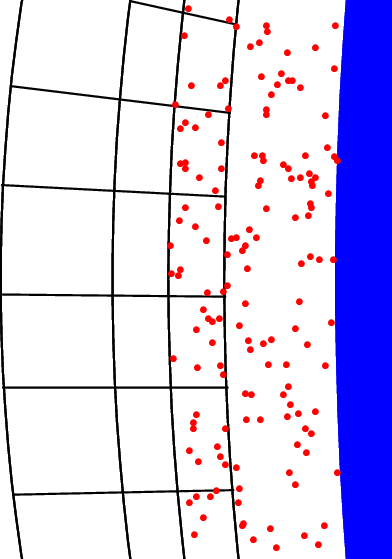
\includegraphics[width=6cm]{../png/pclovm}}
\caption{Handling a plasma sheath adjacent to wall at right.
Plasma has fluid properties discretised using fe indicated using warped grid,
but in sheath is better represented as particles indicated by dots.\label{fig:pcleadj}} 
\end{figure}



%\clearpage
%\section{System 2-7: Interaction between models of different dimensionality} \label{sec:sys2-7}
%\input{sys27}
%\clearpage
%\section{System 2-8: Spatially 3-D plasma kinetic models} \label{sec:sys2-8}
%\input{sys28}
\clearpage
\section{System 3-1: 2-D particle-based model of neutral gas and impurities with critical physics} \label{sec:sys3-1}
The neutrals are represented as super-particles that travel ballistically after introduction
and are lost when they strike the first wall.  In this context, neutral
particle may include photons.
Super-particles have label~$p$, weight~$w_p$ and sample the
point~$({\bf x}_p, {\bf v}_p)$ in 6-D position and velocity space.
At introduction, all particle quantities are defined by sampling
from specified probability distributions.

\subsection{Prerequisites}\label{sec:31prereq}
\subsubsection{Parameters}\label{sec:31param}
It is necessary to have parameters describing initial and boundary conditions.
There must be a means of tying boundary conditions to specific parts
of the surface and volume geometry. See discussion of definitions
of objects/classes for \nep \ in web pages.

\subsubsection{Random number generator}\label{sec:RNG}
It is generally important to test the properties of a random number generator
to ensure there is an absence of bias, typically by producing histograms of
the output and comparing with expected curves. If other routines are found to be unsuitable,
a technique based on the `Mersenne Twister' should give a satisfactory sequence
of pseudo-random numbers. 

For a range of applications where
functions or distributions do not vary on very small scales, Quasi-Monte Carlo
sampling~\cite{niederreiter} may be preferable to Monte Carlo. Note that although the place-name
Monte-Carlo has a hyphen, the name of the mathematical technique does not by convention.
For parallel computation, it will generally be best to compute a block of numbers at a time.

\subsubsection{Sampling from a specified distribution}\label{sec:specdist}
\paragraph{Generally}\label{specdistgen}
Textbooks such as Kalos and Whitlock~\cite{kaloswhitlock} (notable
for its treatment of radiation transport in \S\,6)  explain how to
generate samples of a given distribution $f(x)$ 
from random numbers uniformly sampled on the unit interval. Suppose that
$\xi$ is such a random number, then the corresponding value of $x$ is given by
solution of
\begin{equation}\label{eq:invdistbn}
\xi=1-\int_0^x f(x')dx'
\end{equation}
\Eq{invdistbn} may be solved explicitly for~$x$ in many important cases

\paragraph{Gaussian distribution}\label{sec:specdistgaussian}
This may be sampled using the Box-Muller method~\cite[\S\,3.1]{kaloswhitlock}.
Given two random numbers $\xi_1$ and $\xi_2$ uniformly sampled on the unit
interval, then two samples of a Gaussian distribution $f(x) \propto \exp(-x^2/2)$
are given by
\begin{eqnarray}\label{eq:gaussamp}
&&\sqrt{[-2(\ln(1-\xi_1)]} \cos 2\pi \xi_2 \\
&&\sqrt{[-2(\ln(1-\xi_2)]} \cos 2\pi \xi_1
\end{eqnarray}

\paragraph{Knudsen cosine}\label{sec:specdistknud}
Sample by accept-reject from the Knudsen cosine distribution below~\Eq{distknud} to launch
particle trajectories.

Let $f_{max}$ and $s_{max}$ be the maximum of the distribution function
in $[0,6v_{th,i,Kn})$ and the associated speed, respectively
where $v_{th,i,Kn}=\sqrt{2kT_{Kn}/m_{i}})$. Then provide
pairs of random numbers $R_{f}\in[0,f_{max}]$ and $v_{R}\in[0,6v_{th,i,Kn}]$
(and other components of velocity similarly sampled for the tangential
components (but with a negative velocity ranges)). Keep the particle
with normal speed $v_{R}$ if $R_{f}<f_{n,Kn}(v_{R})$.

\subsection{Sources and sinks of neutrals}\label{sec:31sources}
\subsubsection{Knudsen distribution}\label{sec:Knudsen}
As suggested in the TN-07 Neptune report by Parra, Barnes and Hardman~\cite{2047357-TN-07}
%(\url{https://github.com/ExCALIBUR-NEPTUNE/Documents/blob/main/reports/2047357/TN-07.pdf}
equations (5.9)-(5.13), the source of neutrals emitted from a wall
can be described by the Knudsen cosine distribution
\begin{equation}\label{eq:distknud}
f_{n,Kn}\left(\boldsymbol{v};\boldsymbol{n}\cdot\boldsymbol{v}>0\right)=\frac{3}{4\pi}\left(\frac{m_{i}}{kT_{Kn}}\right)^{2}\frac{\boldsymbol{n}\cdot\boldsymbol{v}}{\left|v\right|}\exp\left(-\frac{m_{i}v^{2}}{2kT_{Kn}}\right)
\end{equation}
where $\boldsymbol{n}$ is the normal to the wall, the Knudsen distribution
is used for outgoing neutrals for which $\boldsymbol{n}\cdot\boldsymbol{v}>0$,
and $kT_{Kn}$ is a parameter that controls the temperature
of the emitted neutral distribution. The Knudsen cosine distribution appears with a factor of
a particle flux in Equation~(5.9) of~\cite{2047357-TN-07}, so
despite the "$f$"~notation, it has different units to the other distributions~$f$.

%Propose that for simplicity we also use a Knudsen cosine distribution
%for the neutrals coming from a gas puff, if needed, at least as a
%starting point.

\subsubsection{Volumetric distribution}\label{sec:voldist}
As a starting point, the source of neutrals should be fixed
in time and given a prescribed spatial distribution around the edge
of the simulation domain. A point source, ie.\ delta function in space, 
would be a valid representation of a `gas valve'. Volumetric sources  consisting
of eg.\ a Maxwellian at a given temperature) could be considered for testing purposes.

\subsubsection{Recycling}\label{sec:recyc}
This cannot be properly treated without coupling to a plasma model,
hence is treated in  \Sec{33recyc}.

\subsubsection{Particle sink}\label{sec:volsink}
An explicit volume pumping region,
where neutrals are absorbed when they reach it. This might be
specified by a set of finite element identifiers~$e$.

\subsection{Boundary condition for neutral particles}\label{sec:bcs}
The particle simulation domain need not coincide with the simulation domain, 
since there may be finite elements where a species is treated as a fluid.
\subsubsection{Perfect Absorption}\label{sec:bcsperf}
Any particles that reach a domain boundary are deleted.
\subsubsection{Reflection}\label{sec:bcsrefl}
These conditions are very useful for testing eg.\ energy conservation. 
Perfect specular reflection might be needed to handle symmetry. Supposing
the unit surface normal is~$\boldsymbol{n}$, if the incident velocity is~$\bf{v}_p$,
then the reflected particle has velocity
\begin{equation}\label{eq:bcsreflvel}
\bf{v}_p=\bf{v}_p-2 (\bf{v}_p.\boldsymbol{n}) \boldsymbol{n}
\end{equation}
\subsubsection{Periodic boundaries}\label{sec:bcsperio}
These conditions are very useful for testing purposes, and required for full
or repeat sections of toroidal geometry. Particles simply leave one end
of the domain and re-enter at the other. In the case of a rectilinear
grid, periodic boundary conditions are easily applied by 
taking the modulus of the coordinate value with respect to the period length.
\subsubsection{Imperfect reflection}\label{sec:bcsimperf}
These conditions are probably most appropriate for photons.
This may be achieved by arranging that a fraction~$(1-R_p)$ of incident
particles are absorbed.  If the particles are allowed different weights, then
simply reduce the weight~$w_p$ of each reflected particle by the particle recycling factor~$R_p$
and its energy consistent with recycling factor~$R_E$.
Sputtering is the ejection of surface atoms by impact of both
energetic ions and neutrals. However, the rates of sputtering by
energetic neutrals are relatively low below~$100$\,eV ~\cite[\S\,9.7]{wesson} and may be negelcted
in an initial investigation.
%Suggest making the choice in the first instance for ease of implementation.

%\subsection{Numerical algorithm\label{subsec:neutral-bc-numerics}\label}\label{sec:XX}


%\subsection{Numerical algorithm}\label{sec:XX}
%
%Already part of plasma fluid model. Future `explicit pumping' option
%would be covered by the boundary conditions for neutral particles,
%section~\ref{subsec:neutral-bc-numerics}\label.

%\clearpage
%\section{System 3-2: 2-D moment-based model of neutral gas & impurities} \label{sec:sys3-2}
%\input{sys32}
%\clearpage
%\section{System 3-3: Interaction with 2-D plasma model when available} \label{sec:sys3-3}
%\subsection{Prerequisites}\label{sec:33prereq}
\subsubsection{Cross-section data input}\label{sec:xsect}
%The ionisation cross-section $\Sigma_{ION}$ for Hydrogen ions as a function of~$T_i$
Cross-section data will be obtained from the ADAS library~\cite{adaswebsite}.
Cross-section data $\langle\sigma v\rangle$ averaged over a Maxwellian velocity distribution suitable for
use by a fluid model of the plasma edge is shown in \Fig{xsects}, from Havlickova~et~al.~\cite{Ha13Benc}.
The dominant relevant reactions affecting both neutrals and plasma in the graph are
\begin{eqnarray}
\mbox{Ionisation (ION)} \;\;\; e^-+ H &\rightarrow& H^+ + e^-+ e^-\\
\mbox{Charge-exchange (EXC)} \;\;\; H + H^+ &\rightarrow& H^+ + H
\end{eqnarray}
\begin{figure}
\centerline{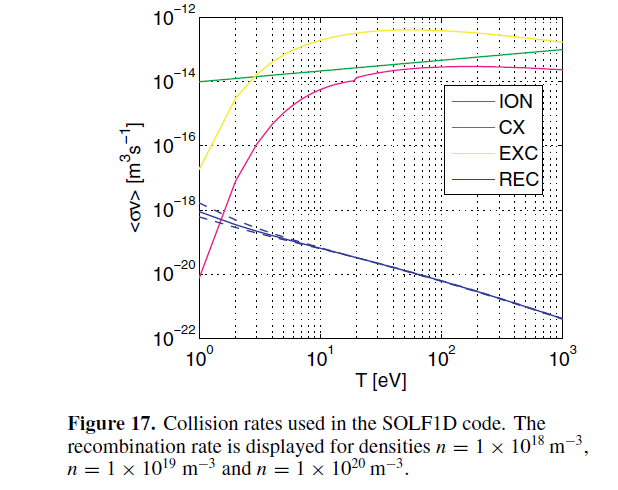
\includegraphics[width=10cm]{../png/Ha13Benc_xsects.png}}
\caption{Extract from publication indicated in the text.  \label{fig:xsects}}
\end{figure}

\subsection{Physical Models}\label{sec:models}
\subsubsection{Introductory model}\label{sec:intromodel}
Perhaps the simplest model to consider is that for ionisation of neutrals by electron impact.
A simple model for ionisation can be written as:
\begin{eqnarray}
\frac{\partial f_{n}}{\partial t} & = & \ldots-R_{ION}n_{i}f_{n}\\
\frac{\partial n_{i}}{\partial t} & = & \ldots+R_{ION}n_{i}n_{n}
\end{eqnarray}
where $R_{ION}$ ($\langle\sigma v\rangle_{ION}$ elsewhere) is a constant ionisation rate, $f_{n}$
is the distribution function for the neutrals, $n_{i}$ and $n_{n}$
are the ion and neutral densities. The quasineutrality assumption implies
$n_{e}=n_{i}$. So the `source term' in the plasma density equation is
\begin{equation}
S_{ION}({\bf x})\equiv R_{ION}n_{i}n_{n}=R_{ION}n_{i}\int d^{3}v\,f_{n}(\boldsymbol{v})
\end{equation}
the integral in which converts, for number densities, into weighted counts of the number
of particles within a given spatial volume about point~${\bf x}$.

\begin{figure}
\centerline{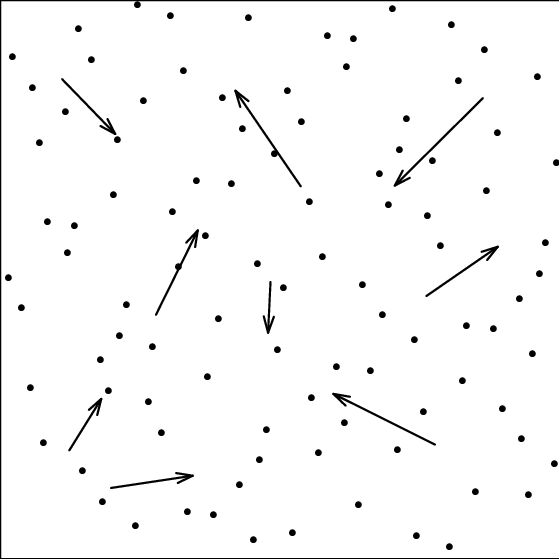
\includegraphics[width=6cm]{../png/harrows.png}}
\caption{Configuration for ionisation.
Neutrals, indicated by arrows, moving against a background of thermal electrons shown
as dots.  \label{fig:harrows}}
\end{figure}
The loss term in the neutral density equation is computed using Monte Carlo
techniques, cf. Verboncouer~\cite{Ve05Part}, configuration sketched in \Fig{harrows}. The probability of ionisation of a
particle at time~$t_n$ travelling with velocity~${\bf v}_p$ in the following
interval of~$\Delta t$ is
\begin{equation}
\mathrm{p}_p(t_n) = 1-\exp\left(-n_e \sigma_{ION} |{\bf v}_p| \Delta t\right)
\end{equation}
where the cross-section for ionisation is $\sigma_{ION}$. Provided the background
density~$n_e$ is approximately constant in space and time, and $\sigma_{ION}$
variation with energy~$\mathcal{E}$ is assumed to be  negligible, taking 
for example
\begin{equation}
\nu_{\sigma max}= \max_{\bf x} \{n_t({\bf x})\}\max_{\mathcal{E}}\{\sigma_T(\mathcal{E}) |{\bf v}|\}
\end{equation}
then for every particle, provided all particles have the same weight (ie.\ identical
superparticles), approximately
\begin{equation}
\mathrm{p}_p =\mathrm{p}_T= 1-\exp\left(-\nu_{\sigma max} t\right)
\end{equation}
and the number of neutrals that undergo ionisation in volume~$\Delta V$
is $\mathrm{p}_T n_n \Delta V$. Such particles should be chosen at random from those
in ~$\Delta V$.

The Monte Carlo algorithm for selecting which neutrals turn into ions, is simple
provided that particles are distributed at random throughout~$\Delta V$, viz.\ to
obtain a random number~$\xi$ from the uniform distribution on the unit interval
(ie.\ $0<\xi<1$) for each particle in turn and if at the $q^{th}$
$\xi<\mathrm{p}_T$ then  the $q^{th}$~particle  is regarded as ionised at time~$t_n$.
If particles are each allowed a weight~$w_p(t)$  which varies with time, then the 
weight of the neutral may simply be reduced to account for the ionisation
\begin{equation}
w_p(t_n+\Delta t)=\mathrm{p}_p(t_n) w_p(t_n)
\end{equation}

\subsubsection{Detailed model}\label{sec:modet}
For sources in the fluid equations due to ionisation of neutrals by electrons, the
formulae, cf. \Eqr{Snn}{SEn} (\cite[Eqs.(34)-(36)]{Ha13Benc}) are
\begin{eqnarray}
\label{eq:Sne} S^n_e&=& N_n N \langle\sigma v\rangle_{ION} \\
\label{eq:Svn} {\bf S}^{\bf v}_n&=&N_n N \langle\sigma v\rangle_{ION} {\bf v}_n \\
\label{eq:Spe} S^p_e&=& -\frac{2}{3} N_n N \langle\sigma v\rangle_{ION} k I_H\\
\label{eq:Spi} S^p_i&=& \frac{2}{3} N_n N \langle\sigma v\rangle_{ION} (\frac{3}{2} kT_n + \frac{1}{2} m_n {\bf v}_n^2 )
\end{eqnarray}

Note that other effects due to charge-exchange and recombination may be deduced from
the equations in \Sec{sources}. Monte Carlo calculation may then proceed using a total
cross-section for all three interactions.
\subsubsection{Simplified model}\label{sec:modsimp}
For an exploratory calculation with the Hermes-3 equations, the ionisation potential term is an unwelcome complication
and the momentum term is assumed not to contribute to the evolution of the vorticity~$\omega$.
Hence \Eqr{Sne}{Spi} above become
\begin{eqnarray}
\label{eq:Snesimp} S^n_e&=& N_n N \langle\sigma v\rangle_{ION} \\
\label{eq:Svnsimp} {\bf S}^{\bf v}_n&=& {\bf 0} \\
\label{eq:Spesimp} S^p_e&=& 0 \\
\label{eq:Spisimp} S^p_i&=& \frac{2}{3} N_n N \langle\sigma v\rangle_{ION} (\frac{3}{2} kT_n + \frac{1}{2} m_n {\bf v}_n^2 )
\end{eqnarray}
Compared to the introductory model in \Sec{intromodel}, spatial variations in
background density and cross-section are handled by the null collision method, see \Sec{33nasimp}.

Introducing the (super-)particles newly ionised in time interval~$\Delta t$, occupying
positions~${\bf x}_p$ with label~$p$ and weight~$w_p$ and interaction~$I$:
\begin{eqnarray}\label{eq:Spartion}
S^{n}_e V^e \Delta t & \approx & \Sigma_{pI} w_p\delta_D({\bf x}-{\bf x}_p) \\
S^{p}_i V^e \Delta t & \approx &\frac{2}{3} m_n \Sigma_{pI} w_p\delta_D({\bf x}-{\bf x}_p) \frac{1}{2} \mathbf{v}_{n,pI}^2
\end{eqnarray}
where the contribution to the energy in a finite element~$e$ is a sum over all particle
interactions~$I$ that have occurred in~$e$. These values are projected
on the finite element basis as for charge assignments
($\delta_D$ is the Dirac delta function) so that they give rise to source terms
\begin{eqnarray}\label{eq:Sfluidion}
S^{n}_e({\bf x}) V^e \Delta t & = & \Sigma_{e,p} w_p\phi_{e,\xi}({\bf x}_p) \phi_{e,\xi}({\bf x}) \\
S^{p}_i({\bf x})  V^e \Delta t & \approx &\frac{1}{3} m_n \Sigma_{e,p} w_p
\mathbf{v}_{n,p}^2 \phi_{e,\xi}({\bf x}_p) \phi_{e,\xi}({\bf x})
\end{eqnarray}
where $\phi_{e,\xi}$ is the expansion basis as a function of global
position~${\bf x}$, ie.\ $\phi_{e,\xi}({\bf x})=\phi_e\left({\boldmath \xi}({\bf x})\right)$,
and the mass matrix has been lumped. %Compare \Eq{Sn} and \Eq{SE} of System 2-3.

\subsection{Initial conditions}\label{sec:33init}
These are defined separately for the fluid (`continuum') species
and the particle species.
\subsection{Boundary conditions}\label{sec:33bcs}
Only conditions coupling both particle and fluid species are
to specified here, otherwise see separate treatments.
\subsubsection{Recycling}\label{sec:33recyc}
Recycling of the plasma reaching the wall implies
that the source of neutrals coming from the target
plates has a flux (and spatial profile) equal to the flux of ions
reaching the target multiplied by some recycling coefficient~$R_p$ (eg.\
a fraction like 0.99).
Recycling is a complicated process~\cite[\S\,9.4]{wesson}
whereby the ions penetrate the solid lattice of the surface, lose
significant energy before neutralising and fraction~$R_p$ reappears
at the surface with a relatively low (below~$5$\,$eV$) temperature.

The flux of ionised plasma from the fluid code is~$n\mathbf{v}$,
which translates into a total incident number of particles~$n|\mathbf{v}|\Delta t \Delta S$,
where $\Delta S$ is the area of surface impacted, which might be taken as
the area of a finite element surface. Thus there are $R_pn|\mathbf{v}|\Delta t \Delta S$
recycled particles to be represented as superparticles. If the superparticles have fixed weight then
it might be necessary to use Monte Carlo to treat `fractional' superparticles, but
simple rounding to the nearest integer should meet larger number cases.
Otherwise, if there is a reference weight~$w_{p0}$ then a set of superparticles
should be launched each with a weight close to this value.
It will be assumed that these `recycled' neutrals are born
with a Cosine-Knudsen distribution at a user-specified temperature~$T_{Kn}$ of a few~$eV$.
(Momentum and energy fluxes given by the fluid code may in a simple approximation
be disregarded.)

\subsection{Calculating particle interactions}\label{sec:33na}
\subsubsection{Classical scattering}\label{sec:classcat}
For interactions in which there is significant momentum or energy
transfer, it is necessary to do a classical scattering problem to
account for the interchange. 

For inelastic collisions between two particle of mass~$m_p$ and velocity~${\bf v}_p$,
$p=1,\;2$, momentum and energy conservation give
\begin{eqnarray}\label{eq:mtmecons}
m_1 {\bf v}_1 + m_2 {\bf v}_2 & = & m_1 {\bf v}^+_1 + m_2 {\bf v}^+_2 \\
m_1 {\bf v}^2_1 + m_2 {\bf v}^2_2 & = & m_1 {\bf v}^{+2}_1 + m_2 {\bf v}^{+2}_2 
\end{eqnarray}
where the velocities ${\bf v}^+_1$ and~${\bf v}^+_2$ at the new time 
are found from the observation that momentum conservation is satisfied if
${\bf v}^+_1 = {\bf v}_1- {\bf p}/m_1,\;\;\;{\bf v}^+_2 = {\bf v}_2- {\bf p}/m_2$
for any~${\bf p}$. Substituting in the energy conservation equation, it follows that
${\bf p}= 2\mu_m ({\bf v}_1- {\bf v}_2)$
where reduced mass
\begin{equation}
\mu_m=\frac{m_1 m_2}{m_1+m_2}
\end{equation}
so that 
\begin{eqnarray}\label{eq:v12+}
{\bf v}^+_1 & = & {\bf v}_1 - 2 \frac{m_2}{m_1+m_2} ({\bf v}_1- {\bf v}_2)\\
{\bf v}^+_2 & = & {\bf v}_2 + 2 \frac{m_1}{m_1+m_2} ({\bf v}_1- {\bf v}_2)
\end{eqnarray}

\subsubsection{Simplified models}\label{sec:33nasimp}
The PIC-MCC software~\cite{Ve05Part} accounts for spatial variations in
background density and cross-section by the null collision method,
also known as `delta-tracking'. This method amounts
to a correction to the introductory model, relying on the maximum property of
the rate~$\nu_{\sigma max}$, whereby the number of collisions is reduced according to
the local value of~$n_e \sigma_{ION}$ in the volume~$\Delta V$ (which volume might well
correspond to that of finite element~$e$). The local value gives a more accurate
estimate for $\mathrm{p}_q$. A second random number~$\xi_2$ is drawn from the uniform
distribution and the neutral remains unchanged if  $\xi_2< \mathrm{p}_T-\mathrm{p}_q$.

\subsubsection{Preferred approach}\label{sec:33naprefer}
The ``Direct Sampling" approach of Brown and Martin~\cite{Br03Dire}
involves the most arithmetic per particle of the
techniques considered, but should generally provide increased accuracy which since the
arithmetic cost is likely dominated by data movement, comes essentially ``free of charge".
Note that the sampling techniques needed to treat all $3$~interactions mentioned above are
common to all, although additional modelling is needed to handle momentum
and energy transfer in some interactions. Comparisons of ``Direct Sampling"
and the algorithm used in PIC-MCC are made in refs~\cite{Li11Rese,Be20Revi}.

\begin{figure}
\centerline{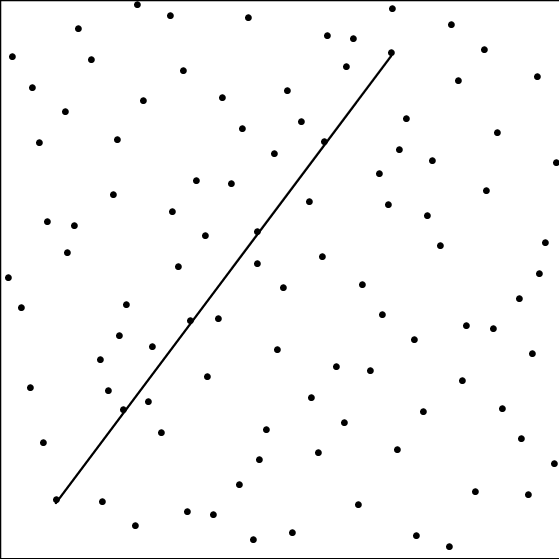
\includegraphics[width=6cm]{../png/hbequisp.png}}
\caption{Conceptual configuration.
A particle, indicated by the straight line, moves against a background thermal (`fluid')
species shown as dots.  In the refinement by De~Esch, interactions take place
at uniformly spaced intervals along the track, also indicated by dots\label{fig:hbequisp}}
\end{figure}

As illustrated in \Fig{hbequisp}, let $\tau (s)$ be the optical depth traversed by a 
article traveling a distance~$s$ through a medium 
with arbitrarily specified macroscopic cross-section~$\sigma(s)$: 
\begin{equation}\label{eq:optd}
\tau(s)= {\int_0}^s \sigma(s')ds'
\end{equation}
We assume only that $\sigma$ is finite and $\sigma(s)\ge 0$. Note that 
\begin{equation}\label{eq:doptd}
\frac{d \tau}{d s} = \sigma (s) 
\end{equation}
To explicitly allow for the case of no collision in a finite distance of travel, 
we define~$\mathrm{P}_{NC}$, the probability of no collisions, as 
\begin{equation}\label{eq:PNC}
\mathrm{P}_{NC} = \exp{(-\tau(\infty))}
\end{equation}
Then the probability density function (pdf) for a collision occurring after a particle has traveled a 
distance~$s$ through the medium is given by~\cite[\S\,7]{lewismiller}
\begin{equation}\label{eq:pdf}
\mathrm{p}(s)=\mathrm{P}_{NC} \delta(s-s_{\infty}) + \frac{d \tau}{d s} \exp{(-\tau(s))}
\end{equation}
where $\frac{d \tau}{d s}$ is the interaction probability per unit distance travelled,
$s_{\infty}$ is the distance to the boundary of the computational domain and
$\exp{(-\tau(s))}$ is the probability of traversing 
distance~$s$ without collision. \Eq{pdf} explicitly allows for cases where 
$\tau(\infty)$ is 
finite, hence there is a possibility of traveling an infinite distance without colliding.

Unbiased random sampling of the Monte Carlo path requires solving the
following for~$s$, distance along the path, 
namely
\begin{equation}\label{eq:xisamp}
\xi = {\int_0}^s \mathrm{p}(s')ds'
\end{equation}
where $\xi$ is sampled from a uniform random variable on~$[0,1)$. In the
spirit of
De~Esch, values of $\xi= j/N_{\xi}, j=1, \ldots N_{\xi}-1$ should be used,
and the charged particle weights (effectively the number of physical
particles each represents) be reduced by~$N_{\xi}$. Values of $N_{\xi} \approx
10-100$ are suggested.
 
In the first step of the sampling, discrete sampling is used to select a collision with probability $(1-\mathrm{P}_{NC})$
or an infinite flight with probability $\mathrm{P}_{NC}$. That is, 
if $\xi > \mathrm{P}_{NC}$, 
then there is a collision. The second step is to sample~$s$ from 
 from the pdf given by:
\begin{equation}\label{eq:partpdf}
g(s')=\frac{1}{G} \frac{d \tau}{d s'}\exp{(-\tau(s'))}
\end{equation}
where
\begin{equation}\label{eq:GPNC}
G= (1-\mathrm{P}_{NC})
\end{equation}
Using \Eq{partpdf}, note that 
\begin{equation}\label{eq:gconstr}
{\int_0}^s g(s')ds' = \frac{1}{G} {\int_0}^{\tau(s)} \exp{(-\tau)}d\tau
\end{equation}
Using \Eqs{xisamp}{partpdf}, we can sample $\tau_s=\tau(s)$ by solving 
\begin{equation}\label{eq:xiG}
\xi=\frac{1}{G} {\int_0}^{\tau_s} \exp{-\tau}d\tau
\end{equation}
This is equivalent to sampling from a truncated exponential pdf, which has 
the solution 
\begin{equation}\label{eq:xiGsoln}
\tau_s -\ln(1-G\xi)
\end{equation}
Pathlength $s$ then follows from \Eq{optd}, viz.
\begin{equation} \label{eq:sfromtau}
\tau_s ={\int_0}^s \sigma(s') ds'
\end{equation}
When $\sigma(s')$ has a simple functional form, \Eq{sfromtau} can often be solved analytically for~$s$. In many 
cases which arise in practice, the solution may involve a transcendental equation or other form 
not amenable to analytic solution. \Eq{sfromtau}, however, can be readily solved numerically for~$s$ 
using Newton iteration with $f= {\int_0}^s \sigma(s') ds' -s$,
starting with an initial estimate $s_0 = \tau_s/\sigma(0)$~\cite{Br03Dire}. 
Because $df/ds\le 0$, $f$ is monotone and there can be at most one root.
For cases where $\sigma(s')\ge 0$,
the Newton iteration is guaranteed to 
converge. However, if $\sigma(s')$ is zero or very small over a portion of the path, $df/ds$~may be~$0$,
leading to numerical difficulties and nonconvergence. This potential problem is 
remedied easily by combining Newton with a bisection search method, such that
bisection is used if $df/ds$ is very small or zero. Using this approach, Brown
and Martin 
found that only $1-5$~iterations are typically needed to converge~$s$ to within
part in $10^6$.
even for extreme variations in $\sigma(s')$. 

 
A final practical point concerns the relation of path length~$s$ to physical coordinates.
If the particle starts at~${\bf x}_0$ and travels in a direction
given by ${\bf v}_p$ parallel to unit vector~${\bf d}$ then the particle path is given by
\begin{equation}\label{eq:patheq}
{\bf x} = {\bf x}_0 + s {\bf d}
\end{equation}
so inverting
\begin{equation}\label{eq:zpatheq}
s = |{\bf x}-{\bf x}_0|/|{\bf d}|
\end{equation}
so it is helpful if ${\bf d}$ is a unit vector.


%\clearpage
%\section{System 3-4: 3-D model of neutral gas & impurities} \label{sec:sys3-4}
%\input{sys34}
%\clearpage
%\section{System 3-5: Interaction with 3-D plasma model} \label{sec:sys3-5}
%\input{sys35}
%\clearpage
%\section{System 3-6: Staged introduction of additional neutral gas/impurity physics} \label{sec:sys3-6}
%\input{sys36}
\clearpage
\section{Summary}\label{sec:summ}
The requirements capture exercise did not raise any significant issues that
had not been anticipated in the Science Plan~\cite{sciplan}.
Concerning modelling and software, there was remarkably little dissension.
The question of the physics to be included has been settled in the
short term  by the need to align with the E-TASC projects on edge modelling.
Longer term there are questions still to be resolved concerning the
details of the gyroaveraged kinetic (or other kinetic) model to be employed,
the inclusion of special relativistic effects, plasma chemistry, 
and for example whether the PFC boundaries should be allowed to `melt',
and whether particle dynamics within the top layers of PFCs should be included.

There is still a debate about how best to deal with situations when the software
even at the Exascale is incapable of resolving boundary or internal layers.
A feature of the lower order (Patankar) fd scheme is that it can be
formulated so that in an implicit time advance of a field advection-diffusion equation,
it acts a contraction mapping on the field, ie.\ it converges to a single, finite solution,
regardless of lack of layer resolution or of size of timestep. Under such circumstances, a spectral
scheme may fail completely cf.\ the dispersion analyses of say Ainsworth et al~\cite{Ai09Disp}
and more recently for spectral/hp element schemes in the Galerkin~\cite{Mo16Eige} and 
discontinuous Galerkin~\cite{Mo15line} contexts,
and users generally prefer an answer to none at all.
Of course, it may be argued that a manifestly erroneous result without an accuracy estimate
will not be used to action large procurements, but in any event it would be better
for the spectral scheme to produce a result at increasingly extreme parameters.

There are a number of ways to achieve this, the most obvious' being the use of
explicit artifical viscosity,
to broaden thinner layers or small features to the
point where full spectral accuracy is achievable.
Different options have been explored, of
which the most robust appears to be `DG-mimicking spectral vanishing viscosity'~ (SVV), see ref~\cite{Mo19Spat}.
Fernandez et al~\cite{Fe19Nonm} specifically addresses robustness when mesh resolution becomes poor..

A better approach from the point-of-view
of accuracy is to insert more resolution (more elements or increased order polynomials)
where aliasing error has been detected. This has its limitations in terms of cost,
but there are also practical issues concerning refinement that still need investigation.
Some of these latter points might be more easily addressed by reformulating the problem 
in terms of a variational approach and/or using the Lie derivative formulation~\cite{La03prac}.
It was anticipated that these could be addressed in the cross-cutting programme.

Interaction with a reactor design framework awaits better definition of data structures
for such tools. There seems no reason however why this should not be addressed inside-out,
as regardless, techniques have to be produced for moving data at the Exascale.

Subject to the above qualifications, the production of proxyapps should proceed in Y2 as indicated
in the Activities Plan~\cite{y12acts}, viz.\ a larger task :
\begin{itemize}
\item to define a referent physics model for the tokamak edge region, accounting
for magnetised plasma behaviour in the presence of significant numbers of neutral atoms and molecules, allowing for
radiation and chemical reactions, and identifying important wall interactions such as sheath formation.
\end{itemize}
This task will be expected to interact with other tasks to ensure feasible implementation.
It is desirable that theroretical support be provided for the EBC pilot code development,
which is a 2-D fluid model, as well as for the 1-D fluid cases with kinetic effects explicitly
listed below.

The candidate algorithms are expected to employ spectral finite element and particle representations.
There are 5 tasks for which advanced mathematical skills will be important:
\begin{enumerate}
\item  to assess performance of spectral elements for \nep \ 
\item  to examine the optimal replacement of plasma species properties
represented on high-order spatially accurate meshes by a particle representation and vice versa.
\item  to study uncertainty quantification (UQ) techniques for \nep \ .
\item  to study model order reduction techniques for \nep \ .
\item  to investigate matrix-preconditioning techniques for \nep \ .
\end{enumerate}
There are 4 tasks to develop proxy-apps for \nep \  of demonstrable, high accuracy
in challenging test-cases, namely :
\begin{enumerate}
\item  2-D model of anisotropic heat transport.
\item  2-D elliptic solver in complex geometry.
\item  1-D fluid solver with simplified physics but with UQ and realistic boundary conditions.
\item  1-D plasma model incorporating velocity space effects.
\end{enumerate}
There are 2  tasks concerning software engineering for \nep \ 
\begin{enumerate}
\item  to investigate DSL and code generation techniques for \nep \ .
\item  to investigate, in collaboration with UKAEA staff, data structures and design patterns for \nep \ .
\end{enumerate}

The Science Plan~\cite{sciplan} shows how the proxyapps should feed into the $5$-year development.
All the tasks may use any identified software packages including
commercial software as part of the demonstration process, provided a feasible route to producing code
freely usable by \nep \  is clearly indicated. It will obviously be better if a task
is linked to the delivery of a proxy-app.




\section*{Acknowledgement}\label{sec:ackn}
\emph{The support of the UK Meteorological Office and Strategic Priorities Fund is acknowledged.}

Valuable input from Ben Dudson is also acknowledged. Stuart Henderson provided helpful
advice concerning plasma radiation.

%\section*{References}
\bibliographystyle{unsrt}
\bibliography{../bib/new,../bib/waynes,../bib/misc,../bib/warv,../bib/neuts,../bib/reac,../bib/exc,../bib/active,../bib/dg1srt}

\appendix
\section{Annex A: Atomic and Molecular Effects}\label{sec:atomic}
%(Phys) How much Tungsten is transported into the hot core by a transient event?
%
%(Phys/EngDes) What amount of noble gas and/or Nitrogen seeding is required to
%enhance the radiative loss enough to protect the divertor?


Often the radiation emitted and absorbed by atoms in different ionisation states 
must be accounted for.
There is a compact introduction in Golub and Pasachoff~\cite[\S\,3.3.1]{golubpasachoff}.
This explains how in principle, given a ``particular mixture of elements at a specified
temperature \ldots the number of atoms per unit volume of the gas which are in a particular
ionisation state may be calculated \ldots then for that atom which emission lines are
emitted"  and so on for all other constituents of the mixture.
(Temperature refers to a black-body radiation field in which the atoms are assumed to sit.)
 ``The sum total of all
these bound-bound emissions, plus the bound-free and free-free emissions" is the spectrum,
where it is explained that `bound' and `free' describe the state of the electron involved
in the formation of the line with respect to the atom.
But ``in practice, carrying out this calculation is \ldots enormously complicated".

The complication follows from the range of competing mechanisms even within atoms
of one element, namely the bound-bound mechanisms of decay and excitation described in
ref~\cite[\S\,3.2.1]{golubpasachoff}, and bound-free
of recombination and photo-emission, because of the different possible degrees of ionisation
as atomic number~$A$ increases and because the proportion of atoms in each ionisation
state depends on the proportions in the others. 


Ambartsumyan~\cite[\S\,5]{ambartsumyan} explains at greater length the
calculation in \emph{thermal equilibrium} of the proportion of different ions for each
element~\cite[\S\,5.2]{ambartsumyan}, then the
bound-free~/~free-bound coefficients~(\S\,5.3---\S\,5.5) and free-free~(\S\,5.6).
In \cite[\S\,24.1--24.2]{ambartsumyan} there is a discussion of metastable
states, which in the astrophysical context are crucial for the formation of forbidden lines in nebulae,
but may also be important in the context of fusion because these metastable atomic
states can survive for many seconds at low densities of matter and of radiation.
By metastable state is meant that no transition to it from lower energy levels
of the electrons is possible except for the so-called `forbidden', less
probable electric quadrupole interactions from the quantum-mechanical matrix elements.

The above outlines the main physics issues. From O'Mullane's slides at the 2008~Summer School~\cite{omullane},
the main difference between astrophysics and fusion
application seems to be that in the plasma context, if it is used, Saha's ionisation
formula needs modification by the Saha-Boltzmann
deviation factors~$b_n$ or `b-factors'~ref~\cite[slide 21]{omullane}.  The Zeeman effect is also neglected,
although this  might be expected to be important,
as from its use in sunspot observation~\cite[\S\,5.2]{brayloughhead} spectral line splitting
by wavelengths of~$0.1$\,nm is expected.

The key observation is from O'Mullane~\cite{omullane}
that in tokamak modelling, there are two distinct
uses for atomic data - (1) to calculate source (loss) terms for species
time evolution equations, and (2) to compute synthetic spectra, ie.\ intensity as a function
of frequency. The latter~(2) is by far the more involved but it is only critical for diagnosticians
working with particular apparatus.
%SH However, it is increasingly being used to develop synthetic diagnostics which are being used to validate simulations.
Indeed, Golub and Pasachoff~\cite[\S\,3.3.2]{golubpasachoff} go on to 
argue that for an optically thin plasma, the radiation (in $W/m^3$)  could be 
expressible as simply as
\begin{equation} \label{eq:erad}
E_R = n_e  n_p  P(T)
\end{equation}
where $n_p$ accounts for the number density of the plasma
ions and $P(T)$ is the emitted power integrated over all wavelengths for a plasma
with a specified mix of elements. 
The separate functions used to compute $P(T)$ depend mainly on electron temperature
with a weak dependence on density. The form of $P(T)$ as a result of the 
integration over spectrum always seems to be smooth. It would seem to
be a prime candidate for precomputation as a function of the fractions of
the major plasma species, and could be approximated very efficiently because
of the smoothness.

O'Mullane~\cite{omullane} give a more
detailed result, namely that
there is a source/sink term for electron energy of form 
\begin{equation} \label{eq:eesource}
S_e=-E_R=n_e \sum_s \sum_{Z=0}^{Z=Z_0(s)} P^Z n^Z -
I^Z \left(\C{S}^{Z\rightarrow Z_p}n^Z+\alpha^{Z_p\rightarrow Z}n^{Z_p}\right)
\end{equation}
where $Z$ is charge state,
the suffix~$s$ on the density has been dropped, $Z_m=Z-1$, $Z_p=Z+1$, and
where $Z_0(s)$ is the number of charge states of species~$s$ included in the model.
It may be inferred that
\begin{eqnarray}
\C{S}^{Z_m\rightarrow Z} \mbox{ or }
\C{S}^{Z\rightarrow Z_p} &=&\mbox{ionisation coefficient}\\
\alpha^{Z\rightarrow Z_m} \mbox{ or }
\alpha^{Z_p\rightarrow Z} &=&\mbox{partial dielectronic recombination rate coefficient}\\
P^Z &=&\mbox{radiated power per atom of $n^Z$}\\
I^Z &=&\mbox{power per atom released in dielectronic recombination}
\end{eqnarray}
where the coefficients, as elsewhere in this section, are expected to be obtained from the
Atomic Data and Analysis Structure~ADAS database~\cite {adaswebsite,openadaswebsite}.
The data requirements for this look relatively modest, assuming the coefficients for
each species and charge state are smooth functions of temperature only. Thus if say
$N_T\approx 20$ samples specify these functions 
and $Z_{sum}=\sum_s Z_0(s)$, then the total number of coefficients required
could be estimated as~$Z_{sum} \times 3 \times N_T \approx 20 \times 3 \times 10 =600$ where
if the number of different elements present $N_s=10$, and
if the average number of charge states $\bar{N}_Z=2$, then $Z_{sum} =N_s \bar{N}_Z \approx 20$.
In another case of interest, a calculation might include only two or three extra species if one were Tungsten~(W),
so $N_s=4$ but then $N_Z=22$ for W~alone if $T_e>40$\,eV~\cite{williamswebsite}.
%\cite[p.\,181]{kayelaby}.

The number densities~$n^Z$ for each charge state may be straightforwardly calculated by
solving a transport equation for each isotope~$n_s$ and using the Saha-Boltzmann formula modified
with b-factors to determine the distribution of charge states. (Further, for heavier elements
a mean atomic mass may be used to avoid separate treatment of isotopic species.)
Much more serious implications for computation~\cite{omullane},
arise in the time evolution equations if each charge state is treated separately.
This may be necessary in a strong electric field because each different ion feels
a different electromagnetic force.
An ion of species~$s$ with charge state~$Z$ will acquire a source
\begin{equation} \label{eq:nzsource}
S_s^Z=\C{S}^{Z_m\rightarrow Z}n_e n^{Z_m} - \left(\alpha^{Z\rightarrow Z_m}+\C{S}^{Z\rightarrow Z_p}\right) n_e n^Z+
\alpha^{Z_p\rightarrow Z} n_e n^{Z_p}
\end{equation}
where again the suffix~$s$ on the density has been dropped. Thus the demands on atomic data
are not very different from those for the energy equation, but 
since the total cost of these additional computations with $Z_0(s)$ extra species will
scale at least as fast as $Z_{sum}=\sum_s Z_0(s)$ (inter-species coupling may add considerably
to the computational expense), rendering negligible
the cost of inputting a few thousand coefficients from disc. In practice a useful
surrogate is produced by replacing separate ionisation states by `superstages'~(slide~17 of ref~\cite{Su06ADAS}),
where one superstage corresponds to one electron shell of the atom. However, even the smaller number of $7$~superstages
required for~W might double or treble the length of a typical computation.

The above is typically as much detail as is sensible to consider under heading~(1).
If detailed diagnostics under~(2) are required, the  generalised collisional-radiative (GCR) model~\cite{Ba03Diel}
gives an idea of the computational demands.
GCR modelling requires each metastable state to be considered separately, since each has a separate finite lifetime.
%SHdo you mean the plasma transport, e.g. parallel or perpendicular, or do you mean from atomic processes? If the latter, then actually the different metastables can have significantly different mean free paths due to differences in ionisation and recombination rate coefficients. 
It helps that the transport of each atom in the state is presumably the same, but even so there is a need to
solve a rate equation for metastable state density at sample points throughout the computational domain
The source terms are complicated, namely for the metastable state labelled~$\rho$
\begin{eqnarray} \label{eq:nrhosource}
S_\rho^Z/n_e&=&\sum_\sigma \C{X}_{\sigma \rightarrow \rho}^{Z\rightarrow Z}n_\sigma
-\sum_\sigma \C{X}_{\rho \rightarrow \sigma}^{Z\rightarrow Z}n_\rho \\
&+&\sum_\mu \C{S}_{\mu \rightarrow \rho}^{Z_m\rightarrow Z}n^{Z_m}_\mu
-\sum_\nu \C{S}_{\rho \rightarrow \nu}^{Z\rightarrow Z_p}n_\rho  \\
&+&\sum_\nu \alpha_{\nu \rightarrow \rho}^{Z_p\rightarrow Z}n^{Z_p}_\nu
-\sum_\mu \alpha_{\rho \rightarrow \mu}^{Z\rightarrow Z_m}n_\rho \\
&+&\sum_\sigma \C{Q}_{\sigma \rightarrow \rho}^{Z\rightarrow Z}n_\sigma
-\sum_\sigma \C{Q}_{\rho \rightarrow \sigma}^{Z\rightarrow Z}n_\rho 
\end{eqnarray}
where the superfix~$Z$ as well as the suffix~$s$ on the density has been dropped
and the new symbols are
\begin{eqnarray}
\C{X}_{\sigma \rightarrow \rho}^{Z\rightarrow Z} &=&\mbox{generalised collisional-radiative (GCR) excitation coefficient} \\
\C{Q}_{\sigma \rightarrow \rho}^{Z\rightarrow Z} &=&\mbox{parent-metastable cross-coupling coefficient}
\end{eqnarray}
\emph{Note that the expressions in both ref~\cite[eq.\ (9)]{Ba03Diel} and ref~\cite[slide 41]{omullane}
appear to contain typos, and that the meanings of $\C{X}$ and $\C{Q}$ have swapped.}
Each of the new terms contains approximately~$8M_Z$ coefficients where $M_Z$ is the number of metastable
states for species~$s$ (which includes the ground state). It may be inferred from refs~\cite{omullane,Su06ADAS}
that the number of metastable states
for a given ionisation~$Z$ is relatively small (slide~9 of ref~\cite{Su06ADAS} indicates that all ionisation
states for Oxygen have $M_z \leq 4$; slide~19 suggests $M_Z\leq6$ for W when $Te<100$\,eV).
%SH This is a bit of an open topic right now, where the number of metastables vary depending on the iso-electronic sequence and the charge of the ion. For some Fe ions, there can be tens of metastables - the open discussion now is how these can be grouped for 2D simulation codes. 
The coefficients~$\C{X}, \C{S}, \C{Q}$ in \Eq{nrhosource} are functions of electron density as well
as temperature so may require at least~$100$ sample points to specify, hence the total data can be estimated
as~$Z_{sum}\times M_Z\times 8M_Z\times 100$.
However FISPACT-II~\cite{Su17FISP} experience with rate equations indicates the cost of 
these additional computations with $M_Z$ metastables far exceeds
the cost of inputting of order ten or so thousand coefficients from disc.

Where the demands of data might become important is in the translation of the $n^Z_\sigma$ into
spectral lines. First the regular excited states, because they equilibrate on the usual
atomic timescales which are negligible compared to plasma timescales, are calculated 
using a purely algebraic relation~\cite[eq.\ (5)]{Ba03Diel},
\begin{equation} \label{eq:niz}
n_i^Z/n_e = \sum_\sigma {^X\C{F}_{i\sigma}} n^Z_\sigma
+ \sum_\mu {^I\C{F}_{i\mu}} n^{Z_m}_\mu
+ \sum_\nu {^R\C{F}_{i\nu}} n^{Z_p}_\nu
\end{equation}
where $^{X,I,R}\C{F}_{i\sigma}$ are the coefficients of excitation, ionisation and recombination
for the transition from metastable state~$\sigma$ to regular excited state~$i$, each is a function
of $n_e$~and~$T_e$ with corresponding storage requirement of order~$100$.
\Eq{niz}  requires $Z_{sum} \times M_S \times M_Z$ $\C{F}$ coefficients where $M_S$ is the number of states,
which is potentially infinite, and indeed in practice could be as large as~$\approx 500$,
necessitating the use of `bundling' of the higher energy states to reduce the number to manageable
proportions, say~$10$~\cite {Ba03Diel}.
Next, as explained in the opening paragraph, to each state there corresponds a description of
its spectrum, which may contain
many separate lines, each described by its wavelength, relative amplitude and
a profile shape which may require several further parameters to describe.
Mitigating the demand for coefficient data, is the fact that the diagnostics need only be
computed intermittently.


%Looking at a 2017 paper by Henderson et al. PPCF 59,055010 which I'll
%admit does give a significant use case, namely protection of the first wall by
%enhanced radiation from noble gas and Nitrogen seeding. However,

To treat atomic physics UQ in a later stage of \nep, a
Monte-Carlo calculation might be considered, involving all the
different interactions between all the metastable states where the Maxwellian
assumption is relaxed, posing a multiscale multiphysics problem.
However, the validity of this approach requires further consideration
as Henderson et al~\cite{He17Opti} also indicates that even as
recently as 2017, errors of 30\,\% were present in important coefficients,
although the discrepancies have now been reduced to approximately~$5$\,\%~\cite{He18Impr}.
%SH This conclusion was only considering line power coefficients. The errors for the ionisation and recombinations are likely >>5%.

%Regarding (1), it requires a lot less data than (2) because only the total intensity of 
%spectral line is needed, not its structure.
%In any event, it seems feasible
%to replace complicated data with averages, so that the amount of data that needs
%to be treated can be matched to the available throughput, whilst keeping within say a 10per cent
%error envelope.
%
%It is also worth pointing out that the problem with metastables arises in astrophysics
%application to both the solar corona and planetary nebulae.
%
%
%With errors of 30per cent around, to say nothing
%of the fact that the electrons will not be Maxwellian as assumed, to me it is
%unnecessary for (1) at least initially to account explicitly for the metastable
%atomic states by means of the rate equations in the Summer School slides, except 
%by means of an overall fudge factor. 
%
%
%Note that the data needed to describe the emission 
%by each metastable state are not large as the formulae for line shape are relatively simple.


\end{document}
